\documentclass[11pt,a4paper]{article}
\usepackage[utf8]{inputenc}
\usepackage{geometry}
\usepackage{graphicx}
\usepackage{array}
\usepackage{booktabs}
\usepackage{longtable}
\usepackage{fancyhdr}
\usepackage{listings}
\usepackage{xcolor}
\usepackage{enumitem}
\usepackage{hyperref}
\usepackage{tabularx}
\usepackage{amssymb}
\usepackage{amsmath}
\usepackage{tikz}
\usetikzlibrary{shapes,arrows,positioning,calc}

% Page layout settings
\geometry{left=1in,right=1in,bottom=1in,top=1.5in,headheight=50pt,headsep=1.5cm}
\setlength{\parindent}{0pt}
\setlength{\parskip}{0.5em}

% Graphics path setting
\graphicspath{{../images/}}

% Listings settings for code blocks
\lstset{
    basicstyle=\ttfamily\small,
    breaklines=true,
    frame=single,
    backgroundcolor=\color{gray!10},
    xleftmargin=0.5cm,
    xrightmargin=0.5cm,
    aboveskip=1em,
    belowskip=1em,
    columns=flexible,
    keepspaces=true,
    showstringspaces=false
}

% Header and footer setup
\pagestyle{fancy}
\fancyhead{}
\fancyfoot{}

% Define header content
\fancyhead[L]{ALS-Dimmer: Adaptive Brightness Control}
\fancyhead[R]{\raisebox{0.15cm}{\includegraphics[width=2.5cm]{logo.png}}}

% Define footer content
\fancyfoot[C]{\thepage}
\fancyfoot[L]{Rev 1.1 -- November 2025}
\fancyfoot[R]{}

% Header/footer lines
\renewcommand{\headrulewidth}{0.4pt}
\renewcommand{\footrulewidth}{0.4pt}

% Hyperref settings
\hypersetup{
    colorlinks=true,
    linkcolor=black,
    urlcolor=blue,
    pdftitle={ALS-Dimmer: Adaptive Brightness Control Design \& Implementation},
    pdfauthor={Albert David}
}

% Custom colors for zones and elements
\definecolor{nightzone}{RGB}{100,150,255}
\definecolor{indoorzone}{RGB}{100,200,100}
\definecolor{outdoorzone}{RGB}{255,180,50}
\definecolor{codeblock}{RGB}{240,240,240}

%------------------------
% Document starts here
%------------------------
\begin{document}
\thispagestyle{fancy}

\vspace*{3cm}

\begin{center}
    {\huge\bfseries ALS-Dimmer}\\[1ex]
    {\Large Adaptive Brightness Control}\\[0.5ex]
    {\Large Design \& Implementation}\\[2ex]
    {\large Author: Albert David}\\[2ex]
    {\large Version 1.1}\\[1ex]
    November 2025\\[2ex]
    {\normalsize A Technical Guide for Display Integration}
\end{center}
\vspace{2em}

\section*{Document Revision History}
\begin{longtable}{|p{0.12\textwidth}|p{0.18\textwidth}|p{0.15\textwidth}|p{0.45\textwidth}|}
    \hline
    \textbf{Version} & \textbf{Date} & \textbf{Author} & \textbf{Description} \\
    \hline
    1.0 & November 9, 2025 & Albert David & Initial release - Complete design specification and implementation guide for adaptive brightness control systems \\
    \hline
    1.1 & November 16, 2025 & Albert David & Minor updates - Updated the document and code to reflect \texttt{MANUAL\_TEMPORARY} state of control loop as read-only \\
    \hline
\end{longtable}

\clearpage

\tableofcontents

\clearpage

%------------------------
% Part I: Fundamentals
%------------------------
\part{Fundamentals of Adaptive Brightness Control}

\section{Introduction}

\subsection{Motivation}

Displays are ubiquitous in modern life -- from smartphones and laptops to automotive in-vehicle infotainment (IVI) systems and home entertainment. However, the ambient light conditions under which these displays operate vary dramatically throughout the day and across different environments. A display that is comfortably readable indoors may become completely invisible in direct sunlight, while a brightness level appropriate for daylight can cause severe eye strain and glare during nighttime use.

\textbf{The challenge:} Human environments span over \textbf{six orders of magnitude} in ambient illuminance -- from dark rooms at night (0.1 lux) to direct sunlight (100,000+ lux). Fixed-brightness displays fail to address this dynamic range, leading to:

\begin{itemize}[noitemsep]
    \item \textbf{Poor visibility} in bright environments (safety hazard in automotive applications)
    \item \textbf{Eye strain and glare} in dark environments (health and comfort issue)
    \item \textbf{Reduced battery life} from unnecessarily high brightness settings
    \item \textbf{Suboptimal user experience} requiring constant manual adjustments
\end{itemize}

\subsection{The Solution: Adaptive Brightness Control}

Adaptive brightness control uses an \textbf{Ambient Light Sensor (ALS)} to continuously monitor environmental illuminance and automatically adjust display brightness to maintain optimal visibility and comfort. This technology is now standard in:

\begin{itemize}[noitemsep]
    \item \textbf{Automotive IVI systems} -- Essential for safety during rapid lighting transitions (tunnels, tree cover, parking structures)
    \item \textbf{Mobile devices} -- Improves battery life and user comfort
    \item \textbf{Laptops and monitors} -- Reduces eye strain during prolonged use
    \item \textbf{Smart home displays} -- Seamless integration with ambient lighting
\end{itemize}

\subsection{Document Scope and Audience}

This document serves two purposes:

\textbf{Part I} provides the \textbf{scientific foundation} for adaptive brightness control:
\begin{itemize}[noitemsep]
    \item Human visual perception and light adaptation physiology
    \item Typical lux ranges in home and automotive environments  
    \item Zone-based mapping strategies for non-linear perception
    \item Curve mathematics (linear vs logarithmic)
    \item Asymmetric response time design principles
\end{itemize}

\textbf{Part II} presents the \textbf{ALS-Dimmer implementation}:
\begin{itemize}[noitemsep]
    \item Hardware-agnostic Linux daemon architecture
    \item Modular sensor and output abstractions
    \item JSON-based configuration system
    \item Control interface for IVI integration
    \item Deployment and testing guidelines
\end{itemize}

\textbf{Target Audience:}
\begin{itemize}[noitemsep]
    \item \textbf{Engineers} implementing ALS-based brightness control for displays
    \item \textbf{Product managers} evaluating adaptive brightness solutions
    \item \textbf{Automotive OEMs} integrating IVI systems
    \item \textbf{Display manufacturers} seeking differentiation features
\end{itemize}

This document assumes basic familiarity with embedded Linux systems, I2C/CAN protocols, and display technologies. No prior knowledge of photometry or human vision is required -- all concepts are explained from first principles with practical engineering focus.

\subsection{Why This Matters}

Properly designed adaptive brightness control is not merely a convenience feature. In automotive applications, it is a \textbf{safety-critical} function:

\begin{itemize}[noitemsep]
    \item \textbf{Tunnel transitions} require rapid brightness increase (dark → bright in $<$2 seconds)
    \item \textbf{Night driving} requires minimal glare to preserve dark-adapted vision
    \item \textbf{Direct sunlight} requires maximum brightness for navigation visibility
\end{itemize}


\section{Ambient Light Environments}

\subsection{Understanding Lux}

\textbf{Lux} (symbol: lx) is the SI unit of illuminance, measuring the amount of luminous flux incident on a surface per unit area. Formally:

\begin{equation}
\text{1 lux} = \frac{1 \text{ lumen}}{\text{m}^2}
\label{eq:lux_definition}
\end{equation}

For practical display engineering, lux can be understood as the \textbf{brightness of the environment} as perceived by a light sensor at the display location. Modern ambient light sensors (like TI OPT4001, Vishay VEML7700) provide direct lux readings with minimal calibration.

\subsection{Typical Lux Ranges}

Understanding real-world illuminance levels is essential for designing effective adaptive brightness algorithms. Table \ref{tab:lux_ranges} summarizes typical lux values across home and automotive environments.

\begin{table}[h]
\centering
\small
\begin{tabular}{|l|r|p{0.45\textwidth}|}
\hline
\textbf{Environment} & \textbf{Lux Range} & \textbf{Notes} \\
\hline
\multicolumn{3}{|c|}{\textbf{Home / Office}} \\
\hline
Dark room at night & 0.1 -- 10 & Moonlight through window, night light \\
\hline
Ambient lighting & 50 -- 150 & Living room, soft lighting \\
\hline
Task lighting & 300 -- 500 & Reading lamp, workspace \\
\hline
Bright office & 500 -- 1000 & Well-lit workspace, fluorescent lighting \\
\hline
\multicolumn{3}{|c|}{\textbf{Automotive}} \\
\hline
Night driving & 0.1 -- 10 & Dashboard + distant streetlights \\
\hline
Parking garage & 10 -- 100 & Artificial lighting, variable quality \\
\hline
Tunnel & 50 -- 500 & Varies by depth/length, rapid transitions \\
\hline
Tree cover / shadows & 500 -- 5000 & Dappled sunlight, highly variable \\
\hline
Overcast day & 1,000 -- 10,000 & Diffuse skylight \\
\hline
Direct sunlight & 10,000 -- 100,000+ & Windshield facing sun, sensor placement critical \\
\hline
\end{tabular}
\caption{Typical lux ranges in home and automotive environments}
\label{tab:lux_ranges}
\end{table}

\subsection{Dynamic Range Challenge}

The most challenging aspect of automotive adaptive brightness is the \textbf{extreme dynamic range}:

\begin{itemize}[noitemsep]
    \item \textbf{Night driving} (1 lux) to \textbf{direct sunlight} (100,000 lux) = \textbf{100,000:1 ratio}
    \item \textbf{Six orders of magnitude} span requires sophisticated algorithms
    \item \textbf{Rapid transitions} (e.g., tunnel entry/exit) require sub-second response
\end{itemize}

Figure \ref{fig:lux_ranges} visualizes these ranges on a logarithmic scale, illustrating why a single linear mapping cannot provide optimal brightness across all conditions.

\begin{figure}[h]
\centering
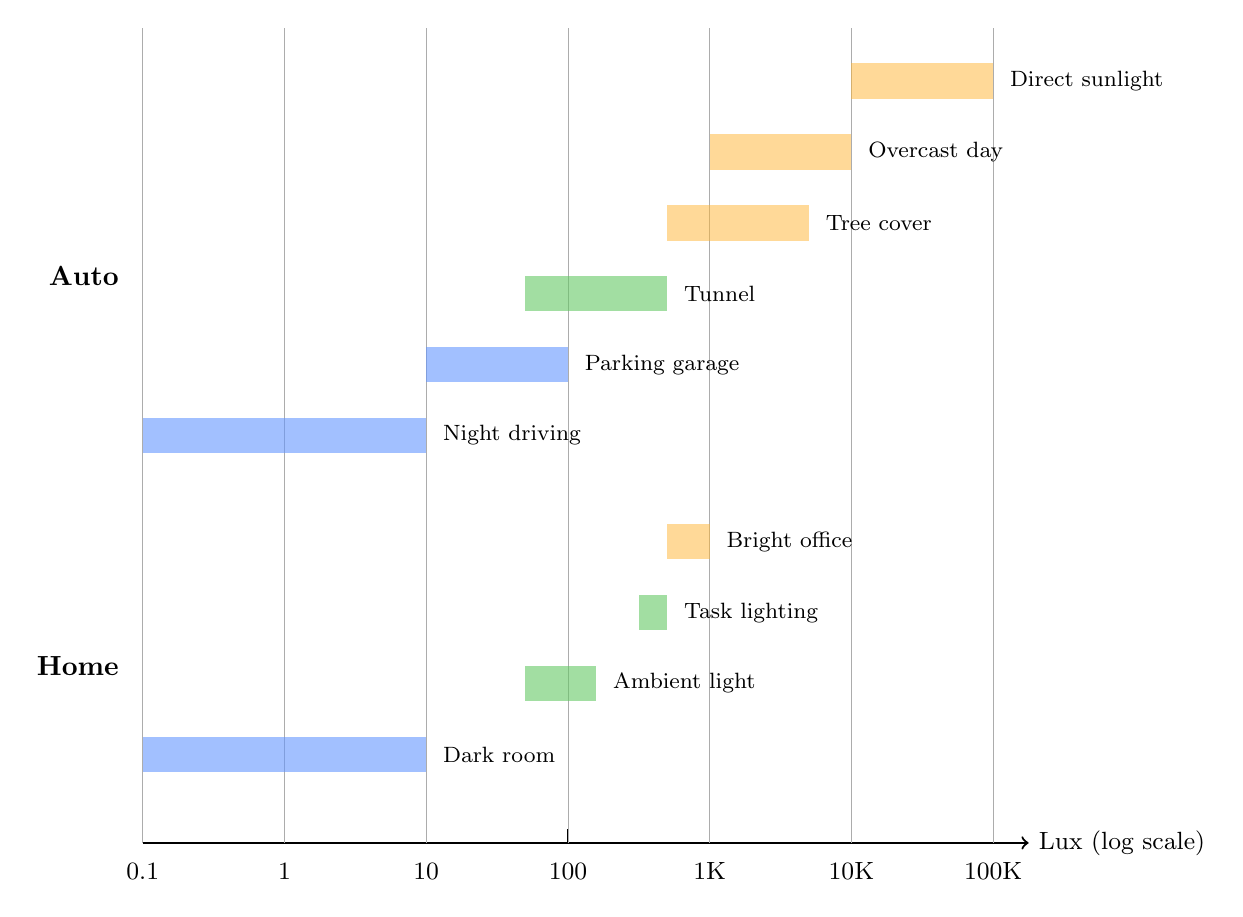
\begin{tikzpicture}[scale=0.9]
    % Logarithmic scale from 0.1 to 100000 lux
    \foreach \x/\label in {0/0.1, 1/1, 2/10, 3/100, 4/1K, 5/10K, 6/100K} {
        \draw (\x*2,0) -- (\x*2,0.2);
        \node at (\x*2,-0.4) {\small \label};
    }
    \draw[thick,->] (0,0) -- (12.5,0) node[right] {\small Lux (log scale)};

    % Vertical gridlines (light gray) for easier alignment
    \foreach \x in {0,1,2,3,4,5,6} {
        \draw[gray!65, very thin] (\x*2,0) -- (\x*2,11.5);
    }

    % Home environments
    % Dark room (0.1-10 lux: x=0 to x=4)
    \fill[nightzone,opacity=0.6] (0,1) rectangle (4,1.5);
    \node[right] at (4.1,1.25) {\footnotesize Dark room};

    % Ambient lighting (50-150 lux: x≈5.4 to x≈6.4)
    \fill[indoorzone,opacity=0.6] (5.4,2) rectangle (6.4,2.5);
    \node[right] at (6.5,2.25) {\footnotesize Ambient light};

    % Task lighting (300-500 lux: x≈7.0 to x≈7.4)
    \fill[indoorzone,opacity=0.6] (7.0,3) rectangle (7.4,3.5);
    \node[right] at (7.5,3.25) {\footnotesize Task lighting};

    % Bright office (500-1000 lux: x≈7.4 to x=8)
    \fill[outdoorzone,opacity=0.5] (7.4,4) rectangle (8,4.5);
    \node[right] at (8.1,4.25) {\footnotesize Bright office};

    % Automotive environments
    % Night driving (0.1-10 lux: x=0 to x=4)
    \fill[nightzone,opacity=0.6] (0,5.5) rectangle (4,6);
    \node[right] at (4.1,5.75) {\footnotesize Night driving};

    % Parking garage (10-100 lux: x=4 to x=6)
    \fill[nightzone,opacity=0.6] (4,6.5) rectangle (6,7);
    \node[right] at (6.1,6.75) {\footnotesize Parking garage};

    % Tunnel (50-500 lux: x≈5.4 to x≈7.4)
    \fill[indoorzone,opacity=0.6] (5.4,7.5) rectangle (7.4,8);
    \node[right] at (7.5,7.75) {\footnotesize Tunnel};

    % Tree cover (500-5000 lux: x≈7.4 to x≈9.4)
    \fill[outdoorzone,opacity=0.5] (7.4,8.5) rectangle (9.4,9);
    \node[right] at (9.5,8.75) {\footnotesize Tree cover};

    % Overcast day (1000-10000 lux: x=8 to x=10)
    \fill[outdoorzone,opacity=0.5] (8,9.5) rectangle (10,10);
    \node[right] at (10.1,9.75) {\footnotesize Overcast day};

    % Direct sunlight (10000-100000 lux: x=10 to x=12)
    \fill[outdoorzone,opacity=0.5] (10,10.5) rectangle (12,11);
    \node[right] at (12.1,10.75) {\footnotesize Direct sunlight};
    
    % Labels
    \node[left] at (-0.2,2.5) {\textbf{Home}};
    \node[left] at (-0.2,8) {\textbf{Auto}};
    
\end{tikzpicture}
\caption{Lux ranges visualization (logarithmic scale)}
\label{fig:lux_ranges}
\end{figure}

\subsection{Implications for Display Design}

These environmental constraints drive several key design requirements:

\begin{enumerate}
    \item \textbf{Sensor placement} must avoid direct light sources while capturing ambient conditions
    \item \textbf{Brightness range} must span from dim (to avoid glare) to maximum panel capability
    \item \textbf{Transition speed} must be asymmetric (fast increase, slow decrease)
    \item \textbf{Zone-based mapping} is essential due to non-linear human perception
\end{enumerate}

The following sections explore the human visual system's response to these conditions and derive optimal control strategies.

\section{Human Visual Perception}

\subsection{Vision Modes}

The human visual system operates in three distinct modes depending on ambient light levels:

\begin{description}
    \item[Photopic vision] ($>$3 cd/m², daylight conditions) -- Mediated by cone cells in the retina, enables color perception and high visual acuity. Optimal for reading, detail work, and color-critical tasks.

    \item[Scotopic vision] ($<$0.01 cd/m², night conditions) -- Mediated by rod cells, provides monochrome vision with high sensitivity to light but poor spatial resolution. Night-adapted eyes can detect very dim sources.
    
    \item[Mesopic vision] (0.01--3 cd/m², twilight) -- Transition range where both rods and cones are active. Most automotive nighttime driving occurs in this range.
\end{description}

For display brightness control, the key insight is that photopic vision (cone-mediated) dominates in all practical use cases except extreme darkness. However, \textbf{adaptation between these modes takes time}, which drives asymmetric transition requirements.

\subsection{Light Adaptation Mechanisms}

The human eye adapts to changing light levels through two primary mechanisms:

\textbf{1. Pupil Response (Fast)}
\begin{itemize}[noitemsep]
    \item \textbf{Constriction} (dark → bright): 100--500 ms
    \item \textbf{Dilation} (bright → dark): 2--5 seconds to noticeably widen, followed by slower chemical processes
    \item Provides ~16:1 dynamic range (2mm to 8mm diameter)
\end{itemize}

\textbf{2. Photochemical Adaptation (Slow)}
\begin{itemize}[noitemsep]
    \item Rhodopsin (rod photopigment) regeneration: 5--30 minutes
    \item Enables vision from starlight to sunlight (~1,000,000:1 range)
    \item Much slower than mechanical pupil response
\end{itemize}

\subsection{The Weber-Fechner Law}

A fundamental principle of human perception states that perceived brightness changes are proportional to the \textbf{logarithm} of the actual physical brightness change:

\begin{equation}
\text{Perceived Brightness} \propto \log(\text{Physical Brightness})
\label{eq:weber_fechner}
\end{equation}

\textbf{Practical implications:}
\begin{itemize}[noitemsep]
    \item Doubling brightness from 10\% to 20\% feels like the same increase as 50\% to 100\%
    \item Linear brightness adjustments feel "wrong" -- large steps at low end, imperceptible at high end
    \item Logarithmic mapping aligns with human perception for optimal user experience
\end{itemize}

\subsection{Asymmetric Adaptation Times}

The most critical insight for display control design:

\begin{center}
\textbf{Dark → Bright adaptation is FAST (pupil constriction)}\\
\textbf{Bright → Dark adaptation is SLOW (pupil dilation + chemistry)}
\end{center}

Table \ref{tab:adaptation_times} quantifies these differences:

\begin{table}[h]
\centering
\begin{tabular}{|l|c|p{0.45\textwidth}|}
\hline
\textbf{Transition} & \textbf{Time} & \textbf{Display Brightness Strategy} \\
\hline
Tunnel exit & 100--500 ms & \textbf{Fast ramp up} (1--2 sec) prevents temporary blindness \\
(Dark → Bright) & (pupil constriction) & Large step sizes, aggressive convergence \\
\hline
Tunnel entry & 2--30 min & \textbf{Slow ramp down} (3--6 sec) prevents glare \\
(Bright → Dark) & (full adaptation) & Small step sizes, gradual convergence \\
\hline
\end{tabular}
\caption{Human adaptation times and display control implications}
\label{tab:adaptation_times}
\end{table}

\subsection{Design Requirements}

These physiological constraints translate to specific engineering requirements:

\begin{enumerate}
    \item \textbf{Logarithmic mapping} in extreme ranges (night/outdoor) to match perception
    \item \textbf{Linear mapping} acceptable in moderate ranges (indoor) for simplicity
    \item \textbf{Asymmetric step sizing}: Large steps for brightening, small for dimming
    \item \textbf{Temporal smoothing}: Prevent rapid oscillations that cause eye strain
    \item \textbf{Minimum brightness}: Never fully black (safety, readability)
    \item \textbf{Maximum brightness}: Panel capability, but consider power/thermal limits
\end{enumerate}

The next section introduces \textbf{zone-based mapping} as the solution that addresses all these requirements simultaneously.

%------------------------
% Section 4: Zone-Based Mapping
%------------------------
\section{Zone-Based Mapping Strategy}

\subsection{The Dynamic Range Challenge}

Real-world display systems must operate across an extraordinarily wide range of ambient light conditions. From dark rooms at night (0.1 lux) to direct sunlight (100,000+ lux), displays must remain readable and comfortable. This represents a dynamic range spanning \textbf{six orders of magnitude}.

Attempting to map this entire range with a single brightness curve inevitably leads to problems:

\begin{itemize}[leftmargin=*]
    \item \textbf{Loss of sensitivity:} Small changes in dim environments go unnoticed
    \item \textbf{Overshooting:} Moderate light changes trigger excessive brightness adjustments
    \item \textbf{Poor usability:} No single curve satisfies both night and day scenarios
    \item \textbf{User frustration:} Constant manual intervention required
\end{itemize}

The fundamental issue is that human perception is \emph{locally linear} but \emph{globally logarithmic}. Within a specific lighting context (e.g., indoor office), small linear adjustments work well. But across vastly different contexts (night vs. day), logarithmic scaling is essential.

\subsection{The Zone-Based Solution}

Rather than using a single curve, the zone-based approach divides the ambient light spectrum into discrete \textbf{zones}, each with its own optimized brightness curve and response characteristics.

\textbf{Key principle:} Each zone handles a manageable subset of the dynamic range where a single curve type (linear or logarithmic) can provide good perceptual uniformity.

\subsubsection{Typical Zone Breakdown}

Most practical implementations use 3-5 zones:

\begin{table}[h]
\centering
\caption{Example Zone Configuration}
\label{tab:zone_config}
\begin{tabular}{@{}lllll@{}}
\toprule
\textbf{Zone} & \textbf{Lux Range} & \textbf{Curve Type} & \textbf{Brightness Range} & \textbf{Use Case} \\
\midrule
Night     & 0--5 lux       & Linear      & 5--20\%   & Dark rooms, nighttime driving \\
Indoor    & 5--500 lux     & Logarithmic & 20--60\%  & Home, office, cloudy day \\
Outdoor   & 500--10,000 lux & Logarithmic & 60--90\%  & Bright day, direct sun \\
Extreme   & 10,000+ lux    & Linear      & 90--100\% & Desert, snow, reflections \\
\bottomrule
\end{tabular}
\end{table}

\subsubsection{Zone Selection Logic}

The system continuously monitors the ambient light sensor and selects the appropriate zone:

\begin{lstlisting}[language=C++, caption={Zone Selection Algorithm (Simplified)}]
Zone selectZone(float lux) {
    if (lux < 5.0) {
        return ZONE_NIGHT;
    } else if (lux < 500.0) {
        return ZONE_INDOOR;
    } else if (lux < 10000.0) {
        return ZONE_OUTDOOR;
    } else {
        return ZONE_EXTREME;
    }
}
\end{lstlisting}

\textbf{Hysteresis:} To prevent oscillation near zone boundaries, implementations typically use hysteresis - requiring the lux value to cross a threshold by a certain margin before switching zones.

\subsection{Benefits of Zone-Based Mapping}

\begin{table}[h]
\centering
\caption{Advantages of Zone-Based vs. Single-Curve Approach}
\label{tab:zone_benefits}
\begin{tabular}{@{}p{0.35\textwidth}p{0.28\textwidth}p{0.28\textwidth}@{}}
\toprule
\textbf{Aspect} & \textbf{Single Curve} & \textbf{Zone-Based} \\
\midrule
Sensitivity in dim light & Poor (compressed) & Excellent (dedicated zone) \\
Handling extreme range & Impossible & Natural (per-zone curves) \\
Perceptual uniformity & Compromised & High (zone-optimized) \\
User intervention & Frequent & Minimal \\
Configuration flexibility & Limited & High (per-zone tuning) \\
Computational cost & Low & Low (simple lookups) \\
\bottomrule
\end{tabular}
\end{table}

\subsection{Zone Transition Smoothing}

To avoid abrupt changes when crossing zone boundaries, most implementations use:

\begin{enumerate}[leftmargin=*]
    \item \textbf{Boundary overlap:} Allow brief co-existence of adjacent zones
    \item \textbf{Gradual transition:} Blend between zone curves near boundaries
    \item \textbf{Rate limiting:} Constrain brightness change rate during transitions
    \item \textbf{Hysteresis bands:} Different thresholds for upward vs. downward transitions
\end{enumerate}

\subsection{Customization Per Use Case}

Zone boundaries and curves should be tailored to the specific application:

\textbf{Automotive IVI:}
\begin{itemize}[leftmargin=*]
    \item Emphasis on nighttime readability (expanded night zone)
    \item Outdoor zone handles 50,000+ lux (dashboard reflections)
    \item Aggressive dimming at night (safety: no distraction)
\end{itemize}

\textbf{Laptop/Mobile:}
\begin{itemize}[leftmargin=*]
    \item Indoor zone covers most usage (5--500 lux)
    \item Battery conservation prioritized in dim zones
    \item User preference learning over time
\end{itemize}

\textbf{Smart Home Display:}
\begin{itemize}[leftmargin=*]
    \item Night zone extends higher (5--20 lux) for bedrooms
    \item Slower transitions (ambient, not safety-critical)
    \item Integration with room lighting controls
\end{itemize}

\subsection{Summary}

Zone-based mapping solves the "impossible problem" of mapping a six order of magnitude dynamic range onto a 0--100\% brightness scale. By dividing the spectrum into manageable zones, each with optimized curves and response times, the system provides:

\begin{itemize}[leftmargin=*]
    \item Excellent sensitivity across all lighting conditions
    \item Natural, perceptually-uniform brightness adjustments
    \item Minimal need for user intervention
    \item Flexibility for application-specific tuning
\end{itemize}

The next section explores the mathematical curves used within each zone.

%------------------------
% Section 5: Brightness Curves
%------------------------
\section{Brightness Curve Mathematics}

Once a zone is selected, the system must map the current lux value to a target brightness percentage. This section presents the two primary curve types used in adaptive brightness control: \textbf{linear} and \textbf{logarithmic}.

\subsection{Linear Curves}

Linear curves provide a straightforward proportional relationship between ambient light and display brightness.

\subsubsection{Formula}

\begin{equation}
B(L) = B_{min} + \frac{B_{max} - B_{min}}{L_{max} - L_{min}} \cdot (L - L_{min})
\label{eq:linear_curve}
\end{equation}

Where:
\begin{itemize}[leftmargin=*]
    \item $B(L)$ = Target brightness (\%) for ambient lux $L$
    \item $B_{min}$ = Minimum brightness for the zone (\%)
    \item $B_{max}$ = Maximum brightness for the zone (\%)
    \item $L_{min}$ = Lower lux boundary of the zone
    \item $L_{max}$ = Upper lux boundary of the zone
    \item $L$ = Current ambient lux reading
\end{itemize}

\subsubsection{Example Calculation}

Consider a \textbf{night zone} with the following parameters:
\begin{itemize}[leftmargin=*]
    \item Lux range: 0--5 lux
    \item Brightness range: 5--20\%
    \item Current ambient: 2.5 lux
\end{itemize}

Applying Equation~\ref{eq:linear_curve}:

\begin{align*}
B(2.5) &= 5 + \frac{20 - 5}{5 - 0} \cdot (2.5 - 0) \\
       &= 5 + \frac{15}{5} \cdot 2.5 \\
       &= 5 + 3 \cdot 2.5 \\
       &= 5 + 7.5 \\
       &= 12.5\%
\end{align*}

\textbf{Result:} At 2.5 lux, the display brightness is set to 12.5\%.

\subsubsection{When to Use Linear Curves}

Linear curves work well when:
\begin{itemize}[leftmargin=*]
    \item The lux range is narrow (1--2 orders of magnitude)
    \item Fine-grained control is needed (e.g., night zones)
    \item Human perception is approximately linear within the range
    \item Predictable, proportional adjustments are desired
\end{itemize}

\subsection{Logarithmic Curves}

Logarithmic curves align with the Weber-Fechner law, providing perceptually uniform adjustments across wide dynamic ranges.

\subsubsection{Formula}

\begin{equation}
B(L) = B_{min} + (B_{max} - B_{min}) \cdot \frac{\log(1 + (L - L_{min}))}{\log(1 + (L_{max} - L_{min}))}
\label{eq:log_curve}
\end{equation}

Where all variables are defined as in Equation~\ref{eq:linear_curve}, and $\log$ denotes the natural logarithm ($\ln$) or base-10 logarithm (both work; base-10 is more intuitive).

\textbf{Implementation Note:} The formula uses $\log(1 + x)$ instead of $\log(L / L_{min})$ for improved numerical stability and to avoid potential edge cases when $L$ approaches $L_{min}$. This shifted logarithm approach maintains the perceptual uniformity property while being more robust in practice.

\subsubsection{Example Calculation}

Consider an \textbf{indoor zone} with:
\begin{itemize}[leftmargin=*]
    \item Lux range: 5--500 lux
    \item Brightness range: 20--60\%
    \item Current ambient: 50 lux
\end{itemize}

Using Equation~\ref{eq:log_curve} with base-10 logarithm:

\begin{align*}
B(50) &= 20 + (60 - 20) \cdot \frac{\log_{10}(1 + (50 - 5))}{\log_{10}(1 + (500 - 5))} \\
      &= 20 + 40 \cdot \frac{\log_{10}(1 + 45)}{\log_{10}(1 + 495)} \\
      &= 20 + 40 \cdot \frac{\log_{10}(46)}{\log_{10}(496)} \\
      &= 20 + 40 \cdot \frac{1.663}{2.696} \\
      &= 20 + 40 \cdot 0.617 \\
      &= 20 + 24.7 \\
      &= 44.7\%
\end{align*}

\textbf{Result:} At 50 lux, brightness is 44.7\%. Note that with the shifted logarithm, 50 lux produces slightly higher brightness than the mathematical midpoint, providing better visibility in the lower-to-mid lux range.

\subsubsection{When to Use Logarithmic Curves}

Logarithmic curves are ideal when:
\begin{itemize}[leftmargin=*]
    \item The lux range spans 2+ orders of magnitude
    \item Perceptual uniformity is critical
    \item The zone covers diverse lighting conditions (e.g., indoor, outdoor)
    \item Alignment with Weber-Fechner law is desired
\end{itemize}

\subsection{Curve Comparison}

Figure~\ref{fig:curve_comparison} illustrates the difference between linear and logarithmic curves for the same lux range (5--500 lux, targeting 20--60\% brightness).

\begin{figure}[ht]
\centering
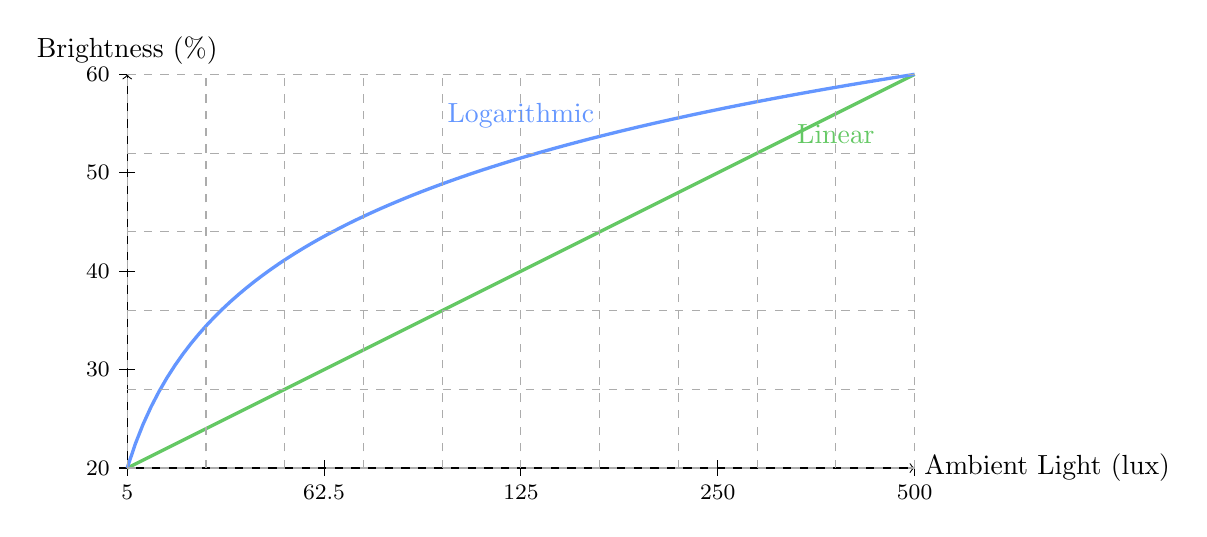
\begin{tikzpicture}[scale=1.0]
    % Axes
    \draw[->] (0,0) -- (10,0) node[right] {Ambient Light (lux)};
    \draw[->] (0,0) -- (0,5) node[above] {Brightness (\%)};

    % Axis labels
    \foreach \x/\label in {0/5, 2.5/62.5, 5/125, 7.5/250, 10/500} {
        \draw (\x,0.1) -- (\x,-0.1) node[below, font=\footnotesize] {\label};
    }
    \foreach \y/\label in {0/20, 1.25/30, 2.5/40, 3.75/50, 5/60} {
        \draw (0.1,\y) -- (-0.1,\y) node[left, font=\footnotesize] {\label};
    }

    % Linear curve (green)
    \draw[indoorzone, very thick] (0,0) -- (10,5) node[pos=0.9, below, indoorzone] {Linear};

    % Logarithmic curve (blue)
    \draw[nightzone, very thick, domain=0:10, samples=100]
        plot (\x, {5 * ln(1 + \x/0.5) / ln(1 + 10/0.5)});

    % Logarithmic label (placed at middle of curve)
    \node[nightzone, above] at (5, 4.2) {Logarithmic};

    % Grid
    \draw[gray!65, dashed] (0,0) grid (10,5);
\end{tikzpicture}
\caption{Linear vs. Logarithmic Curves (5--500 lux $\rightarrow$ 20--60\%)}
\label{fig:curve_comparison}
\end{figure}

\textbf{Observation:} The logarithmic curve provides more sensitivity at lower lux values (steeper slope), which aligns better with human perception in environments transitioning from dim to moderate light.

\subsection{Connection to Weber-Fechner Law}

Recall from Section~3.3 that the Weber-Fechner law states:

\begin{equation}
P \propto \log(S)
\label{eq:weber_fechner_recall}
\end{equation}

Where $P$ is perceived intensity and $S$ is stimulus intensity.

Logarithmic brightness curves directly implement this relationship:
\begin{itemize}[leftmargin=*]
    \item \textbf{Stimulus:} Ambient light (lux)
    \item \textbf{Perceived change:} Display brightness adjustment
    \item \textbf{Result:} Equal percentage changes in lux produce equal perceived brightness changes
\end{itemize}

This is why logarithmic curves feel "natural" to users across wide dynamic ranges, while linear curves can feel too aggressive in bright conditions or too sluggish in dim ones.

\subsection{Practical Curve Selection Guidelines}

\begin{table}[h]
\centering
\caption{Recommended Curve Types by Zone}
\label{tab:curve_selection}
\begin{tabular}{@{}llll@{}}
\toprule
\textbf{Zone} & \textbf{Lux Range} & \textbf{Dynamic Range} & \textbf{Recommended Curve} \\
\midrule
Night         & 0--5 lux          & 1 order (narrow)     & Linear \\
Indoor        & 5--500 lux        & 2 orders (wide)      & Logarithmic \\
Outdoor       & 500--10,000 lux   & 2 orders (wide)      & Logarithmic \\
Extreme       & 10,000+ lux       & 1 order (narrow)     & Linear \\
\bottomrule
\end{tabular}
\end{table}

\subsection{Advanced: Hybrid and Custom Curves}

Some implementations use hybrid approaches:

\begin{itemize}[leftmargin=*]
    \item \textbf{Piecewise curves:} Linear in some sub-ranges, logarithmic in others
    \item \textbf{Exponential curves:} $B(L) = B_{min} \cdot (L / L_{min})^k$ where $k < 1$ for sub-linear growth
    \item \textbf{User-tunable curves:} Allow end users to bias toward dimmer/brighter via a single parameter
    \item \textbf{Learned curves:} Machine learning models that adapt to individual user preferences over time
\end{itemize}

However, the vast majority of practical systems achieve excellent results with the simple linear and logarithmic formulas presented here.

\begin{quote}
\textbf{Hardware transfer assumption:} All equations in this section assume the display exposes a roughly linear 0--100\% control (or that the backlight driver already compensates for its own non-linearity). If a panel's PWM-to-luminance curve is strongly non-linear, add a calibration layer or lookup table so that ``percent'' commands correspond to actual nits; otherwise the lux $\rightarrow$ percent curves here will not yield consistent perceptual changes.
\end{quote}

\subsection{Summary}

Brightness curves translate lux measurements into display brightness percentages. The choice between linear and logarithmic depends on the zone's dynamic range:

\begin{itemize}[leftmargin=*]
    \item \textbf{Narrow ranges (night, extreme):} Linear curves provide intuitive, proportional control
    \item \textbf{Wide ranges (indoor, outdoor):} Logarithmic curves align with human perception
    \item \textbf{Mathematical foundation:} Logarithmic curves implement the Weber-Fechner law
\end{itemize}

The next section addresses how quickly these brightness changes should be applied.

%------------------------
% Section 6: Response Time and Transition Control
%------------------------
\section{Asymmetric Response Time Design}

Calculating the \emph{target} brightness is only half the problem. The other half is determining \emph{how quickly} to transition from the current brightness to the target. This section explains why response speed matters and how asymmetric transition times improve user experience.

\subsection{Why Response Speed Matters}

Instantaneous brightness changes are jarring and uncomfortable. Consider a driver entering a tunnel: if the display instantly jumps from 80\% to 20\% brightness, it creates visual shock and distraction. Conversely, gradual changes can be imperceptibly slow, causing the user to manually intervene.

The ideal transition speed depends on:
\begin{itemize}[leftmargin=*]
    \item \textbf{Magnitude of change:} Larger changes tolerate faster transitions
    \item \textbf{Direction of change:} Brightening vs. dimming (asymmetric)
    \item \textbf{Human adaptation physiology:} Pupil response time, photochemical processes
    \item \textbf{Application context:} Safety-critical (automotive) vs. comfort (home)
\end{itemize}

\subsection{Asymmetric Adaptation: Dark $\rightarrow$ Bright vs. Bright $\rightarrow$ Dark}

Recall from Section~3.3 that human visual adaptation is highly \textbf{asymmetric}:

\begin{table}[h]
\centering
\caption{Asymmetric Transition Time Guidelines}
\label{tab:asymmetric_times}
\begin{tabular}{@{}llll@{}}
\toprule
\textbf{Transition} & \textbf{Pupil Response} & \textbf{Full Adaptation} & \textbf{Recommended Display Speed} \\
\midrule
Dark $\rightarrow$ Bright & 100--500 ms & 1--5 minutes & Fast (200--800 ms) \\
Bright $\rightarrow$ Dark & 100--500 ms & 2--30 minutes & Slow (1--4 seconds) \\
\bottomrule
\end{tabular}
\end{table}

\textbf{Key principle:} Match display transition speed to human adaptation capability.

\begin{itemize}[leftmargin=*]
    \item \textbf{Brightening (dark $\rightarrow$ bright):} Fast transitions are acceptable because:
        \begin{itemize}
            \item Pupils constrict quickly (100--500 ms)
            \item No photochemical delay (cones already active)
            \item Users expect immediate response when more light is available
        \end{itemize}
    \item \textbf{Dimming (bright $\rightarrow$ dark):} Slow transitions are preferred because:
        \begin{itemize}
            \item Photochemical adaptation is slow (minutes to fully adapt)
            \item Premature dimming strains users trying to read the display
            \item Gradual dimming goes unnoticed (comfortable)
        \end{itemize}
\end{itemize}

\subsection{Three-Tier Threshold Algorithm}

The ALS-Dimmer system uses a \textbf{three-tier threshold-based step sizing} algorithm. Rather than calculating steps proportional to error, this approach selects from three fixed step sizes based on error magnitude ranges. This provides precise per-zone control while guaranteeing predictable settling behavior.

\subsubsection{Algorithm Overview}

Define:
\begin{itemize}[leftmargin=*]
    \item $B_{current}$ = Current display brightness (\%)
    \item $B_{target}$ = Target brightness from curve (\%)
    \item $e$ = Error = $B_{target} - B_{current}$
    \item $\Delta B$ = Brightness step size per iteration
    \item $T_{large}$ = Large error threshold (\%)
    \item $T_{small}$ = Small error threshold (\%)
\end{itemize}

\subsubsection{Step Size Selection Logic}

The system maintains \textbf{six asymmetric step sizes per zone}:

\begin{itemize}[leftmargin=*]
    \item \textbf{Large steps:} $\Delta B_{large\text{-}up}$ (brightening), $\Delta B_{large\text{-}down}$ (dimming)
    \item \textbf{Medium steps:} $\Delta B_{medium\text{-}up}$ (brightening), $\Delta B_{medium\text{-}down}$ (dimming)
    \item \textbf{Small steps:} $\Delta B_{small\text{-}up}$ (brightening), $\Delta B_{small\text{-}down}$ (dimming)
\end{itemize}

\begin{equation}
\Delta B =
\begin{cases}
\Delta B_{large\text{-}up} & \text{if } e > T_{large} \text{ (large brightening)} \\
\Delta B_{medium\text{-}up} & \text{if } T_{small} < e \leq T_{large} \text{ (medium brightening)} \\
\Delta B_{small\text{-}up} & \text{if } 0 < e \leq T_{small} \text{ (small brightening)} \\
0 & \text{if } e = 0 \text{ (at target)} \\
-\Delta B_{small\text{-}down} & \text{if } -T_{small} \leq e < 0 \text{ (small dimming)} \\
-\Delta B_{medium\text{-}down} & \text{if } -T_{large} \leq e < -T_{small} \text{ (medium dimming)} \\
-\Delta B_{large\text{-}down} & \text{if } e < -T_{large} \text{ (large dimming)}
\end{cases}
\label{eq:step_size_threshold}
\end{equation}

\textbf{Key principle:} Dimming steps are typically 50\% smaller than brightening steps for the same magnitude category, implementing the asymmetric adaptation principle.

\subsubsection{Typical Default Parameters}

\begin{table}[h]
\centering
\caption{Default Threshold-Based Step Sizes}
\label{tab:default_steps}
\begin{tabular}{@{}llll@{}}
\toprule
\textbf{Category} & \textbf{Error Threshold} & \textbf{Brightening Step} & \textbf{Dimming Step} \\
\midrule
Large   & $|e| > 20\%$ & 6\%  & 3\% \\
Medium  & $5\% < |e| \leq 20\%$ & 3\%  & 1.5\% (rounded to 2\%) \\
Small   & $|e| \leq 5\%$ & 1\%  & 1\% \\
\bottomrule
\end{tabular}
\end{table}

\subsubsection{Example: Brightening Transition}

\textbf{Scenario:} Display at 20\%, target jumps to 60\% (entering sunlight).

\textbf{Parameters:} $T_{large} = 20\%$, $T_{small} = 5\%$, $\Delta B_{large\text{-}up} = 6\%$, $\Delta B_{medium\text{-}up} = 3\%$, $\Delta B_{small\text{-}up} = 1\%$. Iteration period = 100 ms.

\begin{align*}
\text{Iteration 1:} \quad e &= 60 - 20 = 40\% \quad (> T_{large}) \\
\Delta B &= 6\% \\
B_{new} &= 20 + 6 = 26\% \\[0.5em]
\text{Iteration 2:} \quad e &= 60 - 26 = 34\% \quad (> T_{large}) \\
\Delta B &= 6\% \\
B_{new} &= 26 + 6 = 32\% \\[0.5em]
\text{Iteration 3-5:} \quad & \text{Continue with 6\% steps} \\
B_{new} &= 38\%, 44\%, 50\% \\[0.5em]
\text{Iteration 6:} \quad e &= 60 - 50 = 10\% \quad (T_{small} < e \leq T_{large}) \\
\Delta B &= 3\% \\
B_{new} &= 50 + 3 = 53\% \\[0.5em]
\text{Iterations 7-8:} \quad & \text{Continue with 3\% steps} \\
B_{new} &= 56\%, 59\% \\[0.5em]
\text{Iteration 9:} \quad e &= 60 - 59 = 1\% \quad (\leq T_{small}) \\
\Delta B &= 1\% \\
B_{new} &= 60\%
\end{align*}

Total time: 9 iterations $\times$ 100 ms = \textbf{900 ms}. The display reaches the target in under 1 second with predictable, smooth steps.

\subsubsection{Example: Dimming Transition}

\textbf{Scenario:} Display at 60\%, target drops to 20\% (entering tunnel).

\textbf{Parameters:} Same thresholds, $\Delta B_{large\text{-}down} = 3\%$, $\Delta B_{medium\text{-}down} = 2\%$, $\Delta B_{small\text{-}down} = 1\%$. Iteration period = 100 ms.

\begin{align*}
\text{Iteration 1:} \quad e &= 20 - 60 = -40\% \quad (< -T_{large}) \\
\Delta B &= -3\% \\
B_{new} &= 60 - 3 = 57\% \\[0.5em]
\text{Iterations 2-10:} \quad & \text{Continue with 3\% steps (error remains } > T_{large}\text{)} \\
B_{new} &= 54\%, 51\%, \ldots, 30\% \\[0.5em]
\text{Iteration 11:} \quad e &= 20 - 30 = -10\% \quad (-T_{large} \leq e < -T_{small}) \\
\Delta B &= -2\% \\
B_{new} &= 30 - 2 = 28\% \\[0.5em]
\text{Iterations 12-15:} \quad & \text{Continue with 2\% steps} \\
B_{new} &= 26\%, 24\%, 22\%, 20\%
\end{align*}

Total time: 15 iterations $\times$ 100 ms = \textbf{1.5 seconds}. The slower dimming (compared to 900 ms brightening) allows comfortable visual adaptation.

\subsection{Benefits of Threshold-Based Approach}

The three-tier threshold system provides several advantages for zone-based adaptive brightness:

\begin{itemize}[leftmargin=*]
    \item \textbf{Per-zone customization:} Each zone can define radically different step sizes (e.g., night zone: 1\%/2\%/3\%, outdoor zone: 5\%/8\%/12\%)
    \item \textbf{Predictable settling:} Fixed steps guarantee reaching the target without endless micro-adjustments
    \item \textbf{Safety constraints:} Easy to enforce ``never exceed $X\%$ per step'' limits per zone
    \item \textbf{Computational efficiency:} Simple integer comparisons and additions (no floating-point multiplications)
    \item \textbf{Tuning intuitiveness:} Configuration parameters directly correspond to observable behavior
\end{itemize}

\subsection{Alternative: Proportional Error-Based Algorithm}

An alternative approach used in simpler single-zone systems is \textbf{proportional error-based step sizing}:

\begin{equation}
\Delta B =
\begin{cases}
k_{up} \cdot |e| & \text{if } e > 0 \text{ (brightening)} \\
k_{down} \cdot |e| & \text{if } e < 0 \text{ (dimming)} \\
0 & \text{if } e = 0 \text{ (at target)}
\end{cases}
\label{eq:proportional_algorithm}
\end{equation}

Where $k_{up}$ and $k_{down}$ are gain factors (e.g., $k_{up} = 0.25$, $k_{down} = 0.10$).

\textbf{Advantages:} Fewer tuning parameters, mathematically elegant exponential convergence.

\textbf{Disadvantages:} Produces tiny imperceptible steps near convergence (requiring minimum step thresholds), harder to guarantee per-zone maximum step constraints, and less intuitive for zone-specific customization.

For zone-based systems with diverse lighting conditions, the threshold approach provides superior control and predictability.

\subsection{Transition Timing Comparison}

Figure~\ref{fig:transition_timing} illustrates the difference between fast brightening and slow dimming for the same magnitude change.

\begin{figure}[ht]
\centering
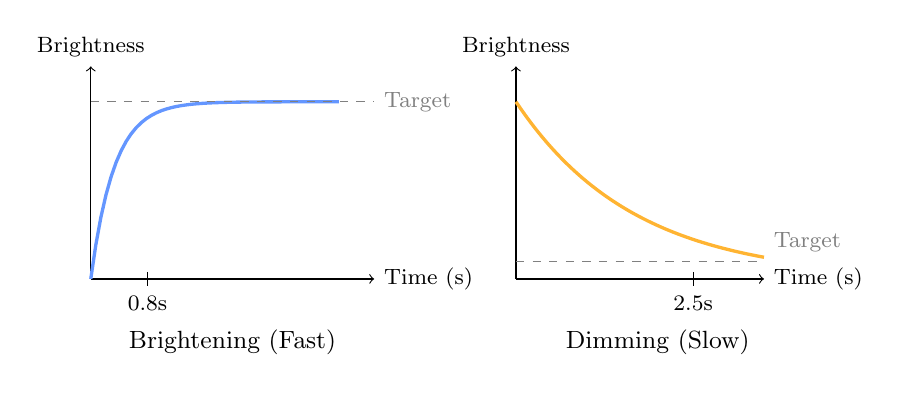
\begin{tikzpicture}[scale=0.9]
    % Brightening plot (left)
    \begin{scope}
        \draw[->] (0,0) -- (4,0) node[right, font=\footnotesize] {Time (s)};
        \draw[->] (0,0) -- (0,3) node[above, font=\footnotesize] {Brightness};
        \draw (2,-0.9) node[font=\small] {Brightening (Fast)};

        % Fast exponential curve
        \draw[nightzone, very thick, domain=0:3.5, samples=50]
            plot (\x, {2.5 * (1 - exp(-3*\x))});

        % Target line
        \draw[dashed, gray] (0,2.5) -- (4,2.5) node[right, font=\footnotesize] {Target};

        % Time markers
        \draw (0.8,0.1) -- (0.8,-0.1) node[below, font=\footnotesize] {0.8s};
    \end{scope}

    % Dimming plot (right)
    \begin{scope}[xshift=6cm]
        \draw[->] (0,0) -- (3.5,0) node[right, font=\footnotesize] {Time (s)};
        \draw[->] (0,0) -- (0,3) node[above, font=\footnotesize] {Brightness};
        \draw (2,-0.9) node[font=\small] {Dimming (Slow)};

        % Slow exponential curve (inverted)
        \draw[outdoorzone, very thick, domain=0:3.5, samples=50]
            plot (\x, {2.5 * exp(-0.6*\x)});

        % Target line (slightly above x-axis)
        \draw[dashed, gray] (0,0.25) -- (3.5,0.25) node[above right, font=\footnotesize] {Target};

        % Time markers
        \draw (2.5,0.1) -- (2.5,-0.1) node[below, font=\footnotesize] {2.5s};
    \end{scope}
\end{tikzpicture}
\caption{Asymmetric Transition Timing: Fast Brightening vs. Slow Dimming}
\label{fig:transition_timing}
\end{figure}

\subsection{Application-Specific Tuning}

Step sizes and thresholds should be adjusted based on use case:

\textbf{Automotive (Safety-Critical):}
\begin{itemize}[leftmargin=*]
    \item Large steps: 8\% (up), 4\% (down) -- driver needs immediate visibility
    \item Medium steps: 4\% (up), 2\% (down) -- moderate transitions
    \item Small steps: 1\% (up/down) -- fine-tuning near target
    \item Thresholds: $T_{large} = 20\%$, $T_{small} = 5\%$
    \item Typical settling time: 0.5--1.0 s (brightening), 1.5--2.5 s (dimming)
\end{itemize}

\textbf{Mobile/Laptop (Battery-Conscious):}
\begin{itemize}[leftmargin=*]
    \item Large steps: 5\% (up), 3\% (down) -- balance responsiveness and battery
    \item Medium steps: 3\% (up), 2\% (down) -- smooth transitions
    \item Small steps: 1\% (up/down) -- preserve battery near target
    \item Thresholds: $T_{large} = 20\%$, $T_{small} = 5\%$
    \item Typical settling time: 1--2 s (brightening), 3--5 s (dimming)
\end{itemize}

\textbf{Smart Home Display (Ambient):}
\begin{itemize}[leftmargin=*]
    \item Large steps: 3\% (up), 2\% (down) -- no urgency, smooth changes
    \item Medium steps: 2\% (up), 1\% (down) -- imperceptible transitions
    \item Small steps: 1\% (up/down) -- ultra-smooth near target
    \item Thresholds: $T_{large} = 15\%$, $T_{small} = 5\%$
    \item Typical settling time: 2--4 s (brightening), 5--10 s (dimming)
\end{itemize}

\subsection{Real-World Performance Validation}

To validate the theoretical concepts presented in this section, we conducted live testing of the ALS-Dimmer system with a responsive configuration optimized for quick transitions. This subsection presents real-world performance data from a hardware test setup.

\subsubsection{Test Configuration}

The test used the following hardware and configuration:

\textbf{Hardware Setup:}
\begin{itemize}[leftmargin=*]
    \item \textbf{Platform:} Raspberry Pi 4
    \item \textbf{Sensor:} Texas Instruments OPT4001 (I$^2$C, address 0x44)
    \item \textbf{Display:} DDC/CI-compatible monitor via I$^2$C
    \item \textbf{Test method:} Manual exposure of sensor to bright LED flashlight (50,000+ lux) followed by sensor covering (near 0 lux), repeated over 230 seconds
\end{itemize}

\textbf{Configuration Parameters (Responsive Profile):}

\begin{table}[h]
\centering
\caption{Test Configuration Parameters}
\label{tab:test_config}
\begin{tabular}{@{}lll@{}}
\toprule
\textbf{Parameter} & \textbf{Value} & \textbf{Notes} \\
\midrule
\multicolumn{3}{l}{\textit{Control Loop Settings}} \\
Update interval & 100 ms & 2$\times$ faster than default \\
Hysteresis & 1.5\% & Reduced for faster zone transitions \\
\midrule
\multicolumn{3}{l}{\textit{Night Zone (0--10 lux)}} \\
Brightness range & 5--30\% & \\
Curve type & Logarithmic & \\
Large steps & 8\% (up), 5\% (down) & 60\% faster than default \\
Medium steps & 4\% (up), 2\% (down) & 100\% faster than default \\
Small steps & 2\% (up), 1\% (down) & 100\% faster than default \\
Thresholds & 15\% (large), 5\% (small) & \\
\midrule
\multicolumn{3}{l}{\textit{Indoor Zone (10--500 lux)}} \\
Brightness range & 30--70\% & \\
Curve type & Linear & \\
Large steps & 12\% (up), 6\% (down) & 50\% faster than default \\
Medium steps & 6\% (up), 3\% (down) & 100\% faster than default \\
Small steps & 2\% (up), 1\% (down) & 100\% faster than default \\
Thresholds & 20\% (large), 6\% (small) & \\
\midrule
\multicolumn{3}{l}{\textit{Outdoor Zone (500--100,000 lux)}} \\
Brightness range & 70--100\% & \\
Curve type & Logarithmic & \\
Large steps & 15\% (up), 8\% (down) & 50\% faster than default \\
Medium steps & 8\% (up), 4\% (down) & 100\% faster than default \\
Small steps & 3\% (up), 2\% (down) & 50\% faster than default \\
Thresholds & 20\% (large), 8\% (small) & \\
\bottomrule
\end{tabular}
\end{table}

\subsubsection{Performance Results}

Figure~\ref{fig:control_loop_response} shows the complete system behavior over a 230-second test period with repeated rapid lighting transitions.

\begin{figure}[p]
\centering
\includegraphics[width=\textwidth]{../images/control-loop-response.jpg}
\caption{\textbf{Real-World Control Loop Performance}\\[0.5em]
Four-panel visualization of ALS-Dimmer adaptive brightness control during stress testing.\\[0.3em]
\textbf{Top panel:} Ambient light (green, left axis) varies from near-0 to 50,000+ lux as sensor is repeatedly exposed to bright light and covered. Target brightness (blue dashed, right axis) is calculated from lux via zone curves. Actual brightness (red solid, right axis) tracks the target with visible lag during dimming transitions.\\[0.3em]
\textbf{Second panel:} Error (blue) shows the difference between target and actual brightness. Step size (red) demonstrates the three-tier threshold algorithm adapting to error magnitude.\\[0.3em]
\textbf{Third panel:} Step category visualization shows the system dynamically selecting large/medium/small steps or settling at target (none). Large steps (red/orange) dominate during rapid transitions; small steps (green/cyan) handle fine-tuning.\\[0.3em]
\textbf{Bottom panel:} Zone transitions between night (blue), indoor (yellow), and outdoor (orange) demonstrate the zone-based mapping strategy handling six orders of magnitude dynamic range.\\[0.3em]
Test configuration: 100ms update interval, responsive step sizes (Table~\ref{tab:test_config}).}
\label{fig:control_loop_response}
\end{figure}

\subsubsection{Key Observations}

The test data validates several theoretical predictions:

\begin{enumerate}[leftmargin=*]
    \item \textbf{Asymmetric response is clearly visible:}
        \begin{itemize}
            \item Brightening transitions (dark $\rightarrow$ bright): Actual brightness tracks target with minimal lag, reaching 90--100\% within 1--2 seconds
            \item Dimming transitions (bright $\rightarrow$ dark): Actual brightness exhibits deliberate lag, taking 3--5 seconds to reach low values, allowing comfortable visual adaptation
        \end{itemize}

    \item \textbf{Three-tier threshold algorithm in action:}
        \begin{itemize}
            \item Large steps (red/orange in panel 3) activate immediately when error exceeds 20\%, providing rapid initial response
            \item Medium steps (yellow/pink) handle mid-range errors (6--20\%), smoothing the approach to target
            \item Small steps (green/cyan) provide fine-tuning when error falls below 6\%
            \item System settles at target (gray ``none'') for extended periods when lux is stable
        \end{itemize}

    \item \textbf{Zone-based operation:}
        \begin{itemize}
            \item Clean transitions between night ($<$10 lux), indoor (10--500 lux), and outdoor (500+ lux) zones
            \item No oscillation or ``zone flapping'' despite 1.5\% hysteresis
            \item Each zone's step sizes are independently optimized (larger steps in outdoor zone for faster response)
        \end{itemize}

    \item \textbf{Error convergence:}
        \begin{itemize}
            \item Error (panel 2, blue line) converges to zero when lux stabilizes
            \item Spike pattern in error correlates directly with manual lighting changes
            \item Step size (panel 2, red line) proportionally responds to error magnitude, validating the threshold-based approach
        \end{itemize}

    \item \textbf{System responsiveness:}
        \begin{itemize}
            \item Despite DDC/CI protocol overhead (~250--300ms per command), the system achieves sub-2-second brightening response
            \item Responsive configuration (100ms update interval, larger steps) provides approximately 2--3$\times$ faster convergence than default settings
            \item The system remains stable with no overshoot or oscillation, even under extreme stress testing
        \end{itemize}
\end{enumerate}

\subsubsection{Comparison to Default Configuration}

The responsive configuration tested here represents an optimized ``fast response'' profile. For comparison:

\begin{itemize}[leftmargin=*]
    \item \textbf{Default configuration:} 200ms update interval, smaller steps, higher thresholds
        \begin{itemize}
            \item Settling time: 4--6 seconds (brightening), 12--18 seconds (dimming)
            \item Use case: Desktop monitors, ambient displays, battery-powered devices
        \end{itemize}
    \item \textbf{Responsive configuration (tested):} 100ms update interval, larger steps, lower thresholds
        \begin{itemize}
            \item Settling time: 1--2 seconds (brightening), 3--5 seconds (dimming)
            \item Use case: Automotive IVI, safety-critical displays, user preference for ``smartphone-like'' feel
        \end{itemize}
\end{itemize}

The test demonstrates that the ALS-Dimmer system successfully balances responsiveness with smoothness, providing fast adaptation to changing lighting conditions while maintaining comfortable, non-jarring transitions.

\subsection{Summary}

Response time is just as critical as target brightness calculation. Key takeaways:

\begin{itemize}[leftmargin=*]
    \item \textbf{Asymmetry is essential:} Fast brightening, slow dimming aligns with human physiology
    \item \textbf{Three-tier threshold algorithm:} Fixed step sizes per error magnitude range provide predictable, zone-customizable transitions
    \item \textbf{Per-zone customization:} Each lighting zone can define optimal step sizes and thresholds
    \item \textbf{Application tuning:} Safety-critical systems use larger steps (faster), ambient systems use smaller steps (smoother)
    \item \textbf{Real-world validation:} Hardware testing confirms theoretical predictions, demonstrating stable, responsive adaptive brightness control across six orders of magnitude dynamic range
\end{itemize}

With zone-based mapping, appropriate curves, and asymmetric threshold-based response timing, Part~I has covered the fundamental principles of adaptive brightness control. Part~II will explore how these concepts are implemented in the ALS-Dimmer system.


\clearpage

%------------------------
% Part II: Implementation
%------------------------
\part{ALS-Dimmer Implementation}

%------------------------
% Section 7: System Architecture
%------------------------
\section{ALS-Dimmer System Architecture}

Having covered the fundamental principles in Part~I, we now turn to the practical implementation of these concepts in the \textbf{ALS-Dimmer} system. ALS-Dimmer is a Linux-Daemon for adaptive brightness control designed for embedded Linux systems, with particular focus on automotive IVI (In-Vehicle Infotainment) applications.

\subsection{Design Philosophy}

ALS-Dimmer is built on three core principles:

\begin{enumerate}[leftmargin=*]
    \item \textbf{Hardware Agnostic:} Support diverse sensors and outputs through factory pattern with interface-based design
    \item \textbf{Configuration-Driven:} No code changes required for different hardware setups
    \item \textbf{Production-Ready:} Robust error handling, logging, systemd integration
\end{enumerate}

\subsection{High-Level Architecture}

Figure~\ref{fig:architecture} shows the main components and data flow:

\begin{figure}[ht]
\centering
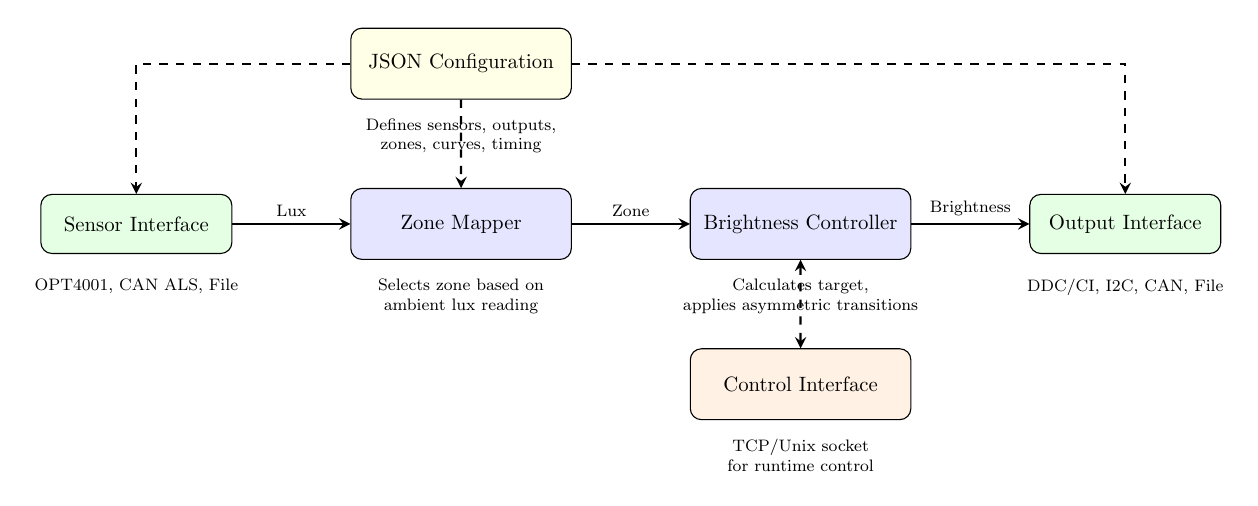
\begin{tikzpicture}[
    scale=0.75,
    every node/.style={transform shape},
    node distance=1.5cm and 2cm,
    block/.style={rectangle, draw, fill=blue!10, text width=3.5cm, text centered, rounded corners, minimum height=1.2cm},
    interface/.style={rectangle, draw, fill=green!10, text width=3cm, text centered, rounded corners, minimum height=1cm},
    arrow/.style={->, >=stealth, thick}
]
    % Sensor layer
    \node[interface] (sensor) {Sensor Interface};
    \node[below=0.3cm of sensor, font=\footnotesize] (sensor_impl) {OPT4001, CAN ALS, File};

    % Zone mapper
    \node[block, right=of sensor] (zonemapper) {Zone Mapper};
    \node[below=0.2cm of zonemapper, font=\footnotesize, text width=3.5cm, align=center] {Selects zone based on\\ambient lux reading};

    % Brightness controller
    \node[block, right=of zonemapper] (controller) {Brightness Controller};
    \node[below=0.2cm of controller, font=\footnotesize, text width=4.0cm, align=center] {Calculates target,\\applies asymmetric transitions};

    % Output layer
    \node[interface, right=of controller] (output) {Output Interface};
    \node[below=0.3cm of output, font=\footnotesize] (output_impl) {DDC/CI, I2C, CAN, File};

    % JSON config (top)
    \node[block, above=1.5cm of zonemapper, fill=yellow!10] (config) {JSON Configuration};
    \node[below=0.2cm of config, font=\footnotesize, text width=4.0cm, align=center] {Defines sensors, outputs,\\zones, curves, timing};

    % Control interface (bottom)
    \node[block, below=1.5cm of controller, fill=orange!10] (control) {Control Interface};
    \node[below=0.2cm of control, font=\footnotesize, text width=3.5cm, align=center] {TCP/Unix socket\\for runtime control};

    % Arrows - main data flow
    \draw[arrow] (sensor) -- node[above, font=\footnotesize] {Lux} (zonemapper);
    \draw[arrow] (zonemapper) -- node[above, font=\footnotesize] {Zone} (controller);
    \draw[arrow] (controller) -- node[above, font=\footnotesize] {Brightness} (output);

    % Config arrows
    \draw[arrow, dashed] (config) -- (zonemapper);
    \draw[arrow, dashed] (config) -| (sensor);
    \draw[arrow, dashed] (config) -| (output);

    % Control arrows
    \draw[arrow, dashed, <->] (control) -- (controller);

\end{tikzpicture}
\caption{ALS-Dimmer High-Level Architecture}
\label{fig:architecture}
\end{figure}

\subsection{Core Components}

\subsubsection{Sensor Interface Layer}

Abstracts ambient light sensor hardware. Implementations include:
\begin{itemize}[leftmargin=*]
    \item \textbf{OPT4001:} TI OPT4001 high-precision I2C sensor (automotive-grade)
    \item \textbf{FPGA-OPT4001:} OPT4001 connected via FPGA I2C bridge
    \item \textbf{CAN ALS:} Sensor data via CAN bus (common in automotive)
    \item \textbf{File Sensor:} Reads lux from file (testing, simulation, integration with external systems)
\end{itemize}

All implementations conform to a common \texttt{SensorInterface} API, allowing hot-swapping via configuration.

\subsubsection{Zone Mapper}

Implements the zone-based mapping strategy described in Section~2.4. Responsibilities:
\begin{itemize}[leftmargin=*]
    \item Monitor current ambient lux reading
    \item Select appropriate zone based on lux boundaries
    \item Apply hysteresis to prevent oscillation
    \item Notify brightness controller of zone changes
\end{itemize}

Zones are fully configurable in JSON, including boundaries, curve types, and brightness ranges.

\subsubsection{Brightness Controller}

Core brightness calculation and transition control logic. Responsibilities:
\begin{itemize}[leftmargin=*]
    \item Calculate target brightness using zone's curve formula
    \item Implement asymmetric error-based step sizing (Section~2.6)
    \item Track current vs. target brightness
    \item Apply rate limiting and smoothing
    \item Handle manual overrides and modes
\end{itemize}

The controller runs in a control loop (typically 100--200 ms period) continuously updating brightness.

\subsubsection{Output Interface Layer}

Abstracts display brightness control hardware. Implementations include:
\begin{itemize}[leftmargin=*]
    \item \textbf{DDC/CI:} Control Display brightness via DDC/CI protocol (VESA standard)
    \item \textbf{I2C Dimmer:} Direct control of LED Driver ICs (e.g FPGA or TCON)
    \item \textbf{CAN Output:} Broadcast brightness via CAN bus to te CAN based Remote Display
    \item \textbf{File Output:} Write brightness to file (testing, integration with external systems)
\end{itemize}

Like sensors, all outputs conform to a common \texttt{OutputInterface} API.

\subsection{Operating Modes}

ALS-Dimmer supports three operating modes:

\begin{table}[h]
\centering
\caption{ALS-Dimmer Operating Modes}
\label{tab:operating_modes}
\small
\begin{tabular}{@{}llp{0.42\textwidth}@{}}
\toprule
\textbf{Mode} & \textbf{Trigger} & \textbf{Behavior} \\
\midrule
AUTO & Default startup & Fully automatic control based on ALS and zones \\
MANUAL & User override via control interface & Brightness fixed at user-specified value. ALS monitoring continues but brightness not updated. \\
MANUAL\_TEMPORARY & User adjustment in AUTO mode & Like MANUAL but reverts to AUTO after timeout (configurable, typically 30--60s). Allows temporary user adjustments without disabling ALS. \\
\bottomrule
\end{tabular}
\end{table}

\textbf{Rationale for MANUAL\_TEMPORARY:} Users may want to temporarily adjust brightness (e.g., reading a map in bright sun) without permanently disabling adaptive control. After a timeout, the system resumes automatic operation. \\
\textbf{Note:} MANUAL\_TEMPORARY mode is a read-only status flag, which reflects a temprory transition phase - it cannot be set through external tcp or unix-domain sockets.

\subsection{Daemon Architecture}

ALS-Dimmer runs as a Linux daemon with the following characteristics:

\begin{itemize}[leftmargin=*]
    \item \textbf{Single-threaded event loop:} Simplifies concurrency, reduces bugs
    \item \textbf{Systemd integration:} Can be managed via \texttt{systemctl} (start, stop, restart)
    \item \textbf{Structured logging:} Configurable log levels (trace, debug, info, warn, error)
    \item \textbf{Graceful shutdown:} Handles SIGINT/SIGTERM cleanly, saves state if needed
    \item \textbf{Hot configuration reload:} For Future extension (currently requires restart)
\end{itemize}

\subsection{Key Design Decisions}

\subsubsection{Why JSON Configuration?}

JSON was chosen over compiled configuration for several reasons:

\begin{itemize}[leftmargin=*]
    \item \textbf{No recompilation:} Hardware changes require only config file edits
    \item \textbf{Tooling:} JSON parsers widely available, easy to validate
    \item \textbf{Human-readable:} Engineers can understand and modify configs
    \item \textbf{Integration:} Easy to generate configs from build systems, provisioning tools
\end{itemize}

\subsubsection{Why Factory Pattern with Interfaces?}

The interface-based factory pattern provides:

\begin{itemize}[leftmargin=*]
    \item \textbf{Modularity:} New sensors/outputs added without touching core logic
    \item \textbf{Testing:} File-based sensors/outputs enable automated testing
    \item \textbf{Portability:} Same core daemon runs on different hardware platforms
    \item \textbf{Maintainability:} Clear separation of concerns
\end{itemize}

\subsubsection{Why Linux Daemon?}

Targeting embedded Linux (especially automotive IVI) drives the daemon architecture:

\begin{itemize}[leftmargin=*]
    \item \textbf{System service:} Runs continuously in background, starts at boot
    \item \textbf{Resource efficient:} Single-threaded, low CPU/memory footprint
    \item \textbf{Standard integration:} Works with systemd, journald, syslog
    \item \textbf{IPC-ready:} Unix Socket Control interface allows integration with HMI frameworks (Android, QNX, etc.)
\end{itemize}

\subsection{Summary}

ALS-Dimmer's architecture embodies the principles described in Part~I through a modular, configuration-driven design. Key strengths:

\begin{itemize}[leftmargin=*]
    \item \textbf{Hardware agnostic:} Supports diverse sensors and outputs
    \item \textbf{Configurable:} Zones, curves, timing all defined in JSON
    \item \textbf{Production-ready:} Systemd integration, robust error handling
    \item \textbf{Testable:} File-based interfaces enable simulation and CI/CD
\end{itemize}

The next sections detail the implementation of each component.

%------------------------
% Section 8: Component Implementation Details
%------------------------
\section{Modular Component Design}

ALS-Dimmer's hardware abstraction is achieved through two key interface hierarchies: \textbf{SensorInterface} and \textbf{OutputInterface}. This section details the design and available implementations.

\subsection{SensorInterface: Ambient Light Sensor Abstraction}

All ambient light sensors implement a common interface with the following contract:

\begin{lstlisting}[language=C++, caption={Sensor Interface (Simplified)}]
class SensorInterface {
public:
    virtual ~SensorInterface() = default;

    // Initialize sensor hardware
    virtual bool initialize() = 0;

    // Read current lux value
    virtual std::optional<float> read_lux() = 0;

    // Check if sensor is operational
    virtual bool is_operational() const = 0;

    // Get sensor name for logging
    virtual std::string get_name() const = 0;
};
\end{lstlisting}

\subsubsection{Available Sensor Implementations}

\paragraph{1. OPT4001 Sensor}

Texas Instruments OPT4001 high-precision I2C light sensor, automotive-grade (-40°C to +125°C).

\textbf{Features:}
\begin{itemize}[leftmargin=*]
    \item 20-bit mantissa + 4-bit exponent (auto-range 0-8), 0.437 µLux to 117,441 lux range (SOT-5X3)
    \item Human eye spectral response matching (photopic filter)
    \item Low power consumption ($<$2 µA standby)
    \item Direct I2C interface (address 0x44 or 0x45)
\end{itemize}

\textbf{Configuration parameters:}
\begin{itemize}[leftmargin=*]
    \item \texttt{i2c\_bus}: I2C bus path (e.g., \texttt{/dev/i2c-1})
    \item \texttt{i2c\_address}: Sensor I2C address (default: \texttt{0x44})
\end{itemize}

\textbf{Hardware Configuration (Validated):}
\begin{itemize}[leftmargin=*]
    \item Register 0x0A: \texttt{0x3239} (auto-range, 100ms conversion, continuous mode)
    \item \textbf{Critical:} Bit 14 (reserved) MUST be 0 per datasheet specification
    \item Initialization wait: 150ms after configuration before first read
    \item Config readback verification recommended to detect hardware rejection
\end{itemize}

\textbf{Note:} Sensor polling rate is controlled globally by \texttt{control.update\_interval\_ms} (typically 200--500ms for OPT4001).

\paragraph{2. FPGA-OPT4001 Sensor}

OPT4001 connected via FPGA I2C bridge. Used when OPT4001 is not directly accessible from CPU's I2C bus (common in automotive SoCs with FPGA co-processors).

\textbf{Differences from direct OPT4001:}
\begin{itemize}[leftmargin=*]
    \item Custom FPGA register interface instead of standard I2C
    \item Sensor data read from FPGA memory-mapped registers
    \item May include FPGA-side filtering/averaging
\end{itemize}

\paragraph{3. CAN ALS Sensor}

Receives ambient light data via CAN bus. Common in automotive systems where ALS is integrated into another ECU (e.g., body control module).

\textbf{Configuration parameters:}
\begin{itemize}[leftmargin=*]
    \item \texttt{can\_interface}: CAN interface name (e.g., \texttt{can0})
    \item \texttt{can\_id}: CAN message ID containing lux data
    \item \texttt{data\_offset}: Byte offset within CAN message
    \item \texttt{scale\_factor}: Multiplier to convert raw value to lux
\end{itemize}

\textbf{Example:} If body module sends lux in CAN ID 0x300, bytes 2--3 (16-bit big-endian), scaled by 0.1:
\begin{lstlisting}[]
"sensor": {
    "type": "can_als",
    "can_interface": "can0",
    "can_id": "0x300",
    "data_offset": 2,
    "scale_factor": 0.1
}
\end{lstlisting}

\paragraph{4. File Sensor (Testing/Integration)}

Reads lux value from a text file. Ideal for:
\begin{itemize}[leftmargin=*]
    \item Automated testing and CI/CD pipelines
    \item Simulation of lighting scenarios
    \item Integration with external systems that write lux to file
\end{itemize}

\textbf{Configuration:}
\begin{lstlisting}[]
"sensor": {
    "type": "file",
    "file_path": "/tmp/ambient_lux.txt"
}
\end{lstlisting}

The file should contain a single floating-point value representing lux.

\subsection{OutputInterface: Display Brightness Control Abstraction}

All display outputs implement a common interface:

\begin{lstlisting}[language=C++, caption={Output Interface (Simplified)}]
class OutputInterface {
public:
    virtual ~OutputInterface() = default;

    // Initialize output hardware
    virtual bool initialize() = 0;

    // Set brightness (0-100)
    virtual bool set_brightness(uint8_t percent) = 0;

    // Get current brightness
    virtual std::optional<uint8_t> get_brightness() = 0;

    // Check if output is operational
    virtual bool is_operational() const = 0;

    // Get output name for logging
    virtual std::string get_name() const = 0;
};
\end{lstlisting}

\subsubsection{Available Output Implementations}

\paragraph{1. DDC/CI Output}

Controls monitor brightness using VESA DDC/CI (Display Data Channel / Command Interface) protocol over I2C.

\textbf{Use cases:}
\begin{itemize}[leftmargin=*]
    \item External monitors connected via HDMI/DisplayPort
    \item Automotive head-up displays with DDC/CI support
    \item Development systems with standard monitors
\end{itemize}

\textbf{Configuration parameters:}
\begin{itemize}[leftmargin=*]
    \item \texttt{i2c\_bus}: I2C bus path (e.g., \texttt{/dev/i2c-5})
    \item \texttt{vcp\_code}: VCP feature code for brightness (default: \texttt{0x10})
\end{itemize}

\paragraph{2. I2C Dimmer Output}

Direct control of LED dimmer ICs(e.g FPGA/TCON) via I2C. Common in automotive instrument clusters.

\textbf{Supported dimmer ICs:}
\begin{itemize}[leftmargin=*]
    \item Generic PWM dimmers with brightness registers
    \item Custom automotive dimmer ICs
\end{itemize}

\textbf{Configuration parameters:}
\begin{itemize}[leftmargin=*]
    \item \texttt{i2c\_bus}: I2C bus path
    \item \texttt{i2c\_address}: Dimmer IC address
    \item \texttt{brightness\_register}: Register address for brightness
    \item \texttt{max\_value}: Maximum register value (for 0--100\% mapping)
\end{itemize}

\paragraph{3. CAN Output}

Broadcasts brightness via CAN bus. Used when display is controlled by another ECU over CAN.

\textbf{Configuration parameters:}
\begin{itemize}[leftmargin=*]
    \item \texttt{can\_interface}: CAN interface name (e.g., \texttt{can0})
    \item \texttt{can\_id}: CAN message ID for brightness command
    \item \texttt{data\_offset}: Byte offset within message
    \item \texttt{scale\_factor}: Multiplier to convert percent to raw value
\end{itemize}

\paragraph{4. File Output (Testing/Integration)}

Writes brightness percentage to a text file.

\textbf{Use cases:}
\begin{itemize}[leftmargin=*]
    \item Automated testing (verify output values)
    \item Integration with external brightness control mechanisms
    \item Debugging and logging
\end{itemize}

\textbf{Configuration:}
\begin{lstlisting}[]
"output": {
    "type": "file",
    "file_path": "/tmp/brightness_output.txt"
}
\end{lstlisting}

The daemon writes brightness as a single integer (0--100) to the file.

\subsection{Modular Architecture Benefits}

The current implementation uses a \textbf{factory pattern} with interface-based design. All sensor and output implementations are compiled into the binary and instantiated at runtime based on JSON configuration.

Figure~\ref{fig:plugin_arch} illustrates the interface hierarchy:

\begin{figure}[ht]
\centering
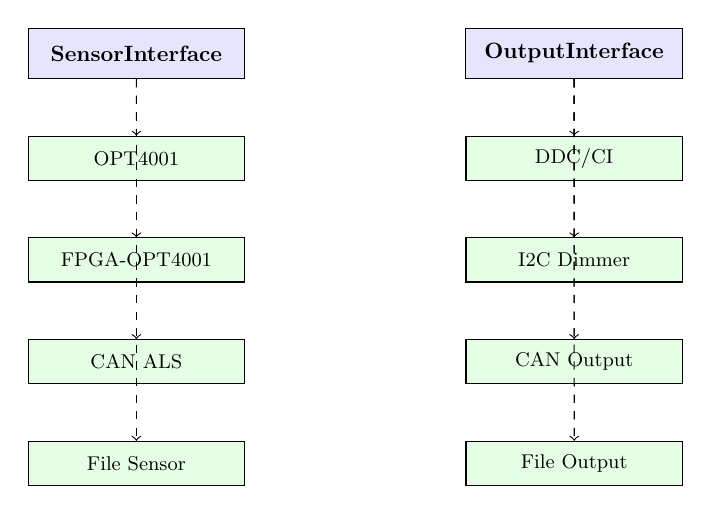
\begin{tikzpicture}[
    scale=0.8,
    every node/.style={transform shape},
    node distance=0.9cm and 3.5cm,
    interface/.style={rectangle, draw, fill=blue!10, text width=3.2cm, text centered, minimum height=0.8cm},
    impl/.style={rectangle, draw, fill=green!10, text width=3.2cm, text centered, minimum height=0.7cm, font=\small},
]
    % Sensor hierarchy
    \node[interface] (sensor_if) {\textbf{SensorInterface}};
    \node[impl, below=of sensor_if] (opt4001) {OPT4001};
    \node[impl, below=of opt4001] (fpga_opt) {FPGA-OPT4001};
    \node[impl, below=of fpga_opt] (can_als) {CAN ALS};
    \node[impl, below=of can_als] (file_sensor) {File Sensor};

    \draw[->, dashed] (sensor_if) -- (opt4001);
    \draw[->, dashed] (sensor_if) -- (fpga_opt);
    \draw[->, dashed] (sensor_if) -- (can_als);
    \draw[->, dashed] (sensor_if) -- (file_sensor);

    % Output hierarchy
    \node[interface, right=of sensor_if] (output_if) {\textbf{OutputInterface}};
    \node[impl, below=of output_if] (ddcci) {DDC/CI};
    \node[impl, below=of ddcci] (i2c_dimmer) {I2C Dimmer};
    \node[impl, below=of i2c_dimmer] (can_out) {CAN Output};
    \node[impl, below=of can_out] (file_output) {File Output};

    \draw[->, dashed] (output_if) -- (ddcci);
    \draw[->, dashed] (output_if) -- (i2c_dimmer);
    \draw[->, dashed] (output_if) -- (can_out);
    \draw[->, dashed] (output_if) -- (file_output);

\end{tikzpicture}
\caption{Modular Architecture: Interface Hierarchies}
\label{fig:plugin_arch}
\end{figure}

\textbf{Key advantages of the factory pattern:}

\begin{enumerate}[leftmargin=*]
    \item \textbf{Decoupling:} Core logic independent of hardware specifics
    \item \textbf{Extensibility:} New sensors/outputs added by implementing interface and updating factory
    \item \textbf{Testability:} File-based implementations enable unit tests and CI/CD
    \item \textbf{Configurability:} Hardware selection at runtime via JSON (no config changes in code)
\end{enumerate}

\textbf{Note on Future Enhancement:} While the current implementation uses a factory pattern with static compilation, the interface design enables future migration to a true \textbf{plugin architecture} with dynamic loading (shared libraries). This would allow adding new sensor/output types without recompiling the daemon.

\subsection{Error Handling and Resilience}

All sensor and output implementations include robust error handling:

\begin{itemize}[leftmargin=*]
    \item \textbf{Initialization failures:} Logged and reported; daemon continues with degraded mode if possible
    \item \textbf{Transient read errors:} Retried with backoff; use last known good value
    \item \textbf{Persistent failures:} Mark component as non-operational; alert via logging
    \item \textbf{Graceful degradation:} If sensor fails, hold last brightness; if output fails, log error but continue operation
\end{itemize}

\subsection{Summary}

The modular architecture provides:
\begin{itemize}[leftmargin=*]
    \item \textbf{4 sensor types:} OPT4001, FPGA-OPT4001, CAN ALS, File
    \item \textbf{4 output types:} DDC/CI, I2C Dimmer, CAN, File
    \item \textbf{Clean interfaces:} Uniform API for all implementations
    \item \textbf{Runtime configuration:} JSON-driven hardware selection
    \item \textbf{Test-friendly:} File-based implementations for automated testing
\end{itemize}

The next section explores the zone controller and brightness calculation logic.

%------------------------
% Section 9: Zone Controller and Brightness Control Loop
%------------------------
\section{Zone Controller and Control Loop}

This section describes how the zone mapper and brightness controller integrate to form the adaptive brightness control loop.

\subsection{Control Loop Overview}

ALS-Dimmer operates in a continuous control loop with the following structure:

\begin{lstlisting}[language=C++, caption={Main Control Loop -- Simplified AUTO Mode (Pseudocode)}]
while (running) {
    // 1. Read ambient light sensor
    lux = sensor->readLux();

    if (lux >= 0) {  // Valid reading
        // 2. Map lux to target brightness using zone
        target = zone_mapper->mapLuxToBrightness(lux);
        current_zone = zone_mapper->selectZone(lux);

        // 3. Calculate smooth transition to target
        current = output->getCurrentBrightness();
        next = brightness_controller->calculateNextBrightness(
            target, current, current_zone);

        // 4. Update display output
        output->setBrightness(next);
    }

    // 5. Sleep until next iteration
    sleep(update_interval_ms);  // typically 200-500 ms
}
\end{lstlisting}

\textbf{Note:} This pseudocode focuses on the core AUTO mode brightness adaptation logic. The actual implementation includes additional features omitted here for clarity: (1)~operating mode handling (AUTO/MANUAL/MANUAL\_TEMPORARY, see Section~9.4), (2)~control interface command processing (see Section~11), (3)~MANUAL\_TEMPORARY timeout checking, and (4)~state management. Method names shown match the actual C++ implementation.

\subsection{Zone Mapper Implementation}

The zone mapper maintains the current active zone and handles transitions.

\subsubsection{Zone Selection Logic}

\begin{lstlisting}[language=C++, caption={Zone Selection with Hysteresis}]
const Zone* ZoneMapper::selectZone(float lux) const {
    // If hysteresis enabled, check if we should stay in current zone
    if (current_zone_ && hysteresis_percent_ > 0.0f) {
        float lux_min = current_zone_->lux_range[0];
        float lux_max = current_zone_->lux_range[1];

        // Calculate hysteresis margins
        float margin_lower = lux_min * hysteresis_percent_ / 100.0f;
        float margin_upper = lux_max * hysteresis_percent_ / 100.0f;

        // Expand boundaries by hysteresis margin
        if (lux >= (lux_min - margin_lower) &&
            lux < (lux_max + margin_upper)) {
            return current_zone_;  // Stay in current zone
        }
    }

    // Find new zone based on lux value
    const Zone* previous_zone = current_zone_;
    for (const auto& zone : zones_) {
        if (lux >= zone.lux_range[0] && lux < zone.lux_range[1]) {
            current_zone_ = &zone;

            // Log zone transition
            if (previous_zone && previous_zone != current_zone_) {
                LOG_INFO("Zone transition: " << previous_zone->name
                         << " -> " << zone.name << " (lux=" << lux << ")");
            }
            return current_zone_;
        }
    }

    // Fallback: use last zone
    current_zone_ = &zones_.back();
    return current_zone_;
}
\end{lstlisting}

\textbf{Key features:}
\begin{itemize}[leftmargin=*]
    \item \textbf{Hysteresis:} Optional feature to prevent oscillation near zone boundaries. Configured via \texttt{control.hysteresis\_percent} (0 = disabled, 5--15 typical for automotive use). When disabled (default: 0), zone selection uses direct boundary checks.
    \item \textbf{Logging:} Zone transitions logged for debugging and analytics
    \item \textbf{Fallback:} Graceful handling if lux falls outside all zones
\end{itemize}

\clearpage

\subsubsection{Zone Configuration Structure}

Each zone is defined by the following parameters:

\begin{table}[h]
\centering
\caption{Zone Configuration Parameters}
\label{tab:zone_params}
\begin{tabular}{@{}llp{0.4\textwidth}@{}}
\toprule
\textbf{Parameter} & \textbf{Type} & \textbf{Description} \\
\midrule
\texttt{name} & String & Human-readable zone identifier \\
\texttt{lux\_range} & Float[2] & Lux boundaries [min, max] (min inclusive, max exclusive) \\
\texttt{brightness\_range} & Int[2] & Brightness range [min, max] (0--100) \\
\texttt{curve} & String & \texttt{linear} or \texttt{logarithmic} \\
\midrule
\multicolumn{3}{@{}l@{}}{\textit{Step sizes (asymmetric for human vision adaptation):}} \\
\texttt{large\_up} & Integer & Large step size for brightening (default: 10) \\
\texttt{medium\_up} & Integer & Medium step size for brightening (default: 4) \\
\texttt{small\_up} & Integer & Small step size for brightening (default: 2) \\
\texttt{large\_down} & Integer & Large step size for dimming (default: 5) \\
\texttt{medium\_down} & Integer & Medium step size for dimming (default: 2) \\
\texttt{small\_down} & Integer & Small step size for dimming (default: 1) \\
\midrule
\multicolumn{3}{@{}l@{}}{\textit{Error thresholds (determine which step size to use):}} \\
\texttt{threshold\_large} & Integer & Error above which large steps used (default: 30) \\
\texttt{threshold\_small} & Integer & Error below which small steps used (default: 10) \\
\bottomrule
\end{tabular}
\end{table}

\textbf{Note:} Asymmetric step sizes implement safety-critical dimming behavior: brightening is ~2× faster than dimming to match human vision adaptation (light adaptation: 1--2 min, dark adaptation: 20--30 min).

\subsection{Brightness Controller Implementation}

The brightness controller calculates target brightness and manages transitions.

\subsubsection{Target Brightness Calculation}

The ZoneMapper calculates target brightness using curve-specific methods:

\begin{lstlisting}[language=C++, caption={Linear Brightness Calculation}]
int ZoneMapper::calculateLinear(float lux, const Zone& zone) const {
    float lux_min = zone.lux_range[0];
    float lux_max = zone.lux_range[1];
    int bright_min = zone.brightness_range[0];
    int bright_max = zone.brightness_range[1];

    // Clamp lux to zone range
    float lux_clamped = std::max(lux_min, std::min(lux, lux_max));

    // Linear interpolation
    float lux_range = lux_max - lux_min;
    if (lux_range <= 0.0f) {
        return bright_min;  // Avoid division by zero
    }

    float normalized = (lux_clamped - lux_min) / lux_range;
    int brightness = bright_min +
        static_cast<int>(normalized * (bright_max - bright_min));

    // Clamp to valid brightness range
    return std::max(0, std::min(100, brightness));
}
\end{lstlisting}

\begin{lstlisting}[language=C++, caption={Logarithmic Brightness Calculation}]
int ZoneMapper::calculateLogarithmic(float lux, const Zone& zone) const {
    float lux_min = zone.lux_range[0];
    float lux_max = zone.lux_range[1];
    int bright_min = zone.brightness_range[0];
    int bright_max = zone.brightness_range[1];

    // Clamp lux to zone range
    float lux_clamped = std::max(lux_min, std::min(lux, lux_max));

    // Logarithmic mapping using log(1 + x) to avoid log(0)
    float lux_offset = lux_clamped - lux_min;
    float lux_range = lux_max - lux_min;

    if (lux_range <= 0.0f) {
        return bright_min;  // Avoid division by zero
    }

    // Add 1 to avoid log(0), then normalize
    float normalized = std::log(1.0f + lux_offset) /
                       std::log(1.0f + lux_range);
    int brightness = bright_min +
        static_cast<int>(normalized * (bright_max - bright_min));

    // Clamp to valid brightness range
    return std::max(0, std::min(100, brightness));
}
\end{lstlisting}

\textbf{Key features:}
\begin{itemize}[leftmargin=*]
    \item \textbf{Curve-specific methods:} Separate implementations for linear and logarithmic curves
    \item \textbf{Safe logarithmic formula:} Uses $\log(1 + x)$ to avoid $\log(0)$ issues and numerical instability
    \item \textbf{Error handling:} Division-by-zero protection for malformed zone configurations
    \item \textbf{Range clamping:} Final brightness clamped to valid [0, 100] range
\end{itemize}

\subsubsection{Asymmetric Transition Control}

The brightness controller implements asymmetric step sizing to match human vision adaptation physiology: fast brightening (light adaptation: 1--2 min) and slow dimming (dark adaptation: 20--30 min, safety-critical for automotive use).

\begin{lstlisting}[language=C++, caption={Asymmetric Step Selection}]
int BrightnessController::getStepSize(int error, const Zone* zone) const {
    int abs_error = std::abs(error);
    bool brightening = (error > 0);

    // Get thresholds and step sizes from zone, or use defaults
    int threshold_large, threshold_small;
    int step_large, step_medium, step_small;

    if (zone) {
        threshold_large = zone->error_thresholds.large;
        threshold_small = zone->error_thresholds.small;

        // Use asymmetric step sizes based on direction
        if (brightening) {
            step_large = zone->step_sizes.large_up;
            step_medium = zone->step_sizes.medium_up;
            step_small = zone->step_sizes.small_up;
        } else {
            step_large = zone->step_sizes.large_down;
            step_medium = zone->step_sizes.medium_down;
            step_small = zone->step_sizes.small_down;
        }
    } else {
        // Simple mode defaults - apply 2:1 asymmetry for safety
        threshold_large = DEFAULT_THRESHOLD_LARGE;  // 20
        threshold_small = DEFAULT_THRESHOLD_SMALL;  // 5
        if (brightening) {
            step_large = 5;
            step_medium = 2;
            step_small = 1;
        } else {
            step_large = 2;  // 50% slower
            step_medium = 1;
            step_small = 1;
        }
    }

    // Select step size based on error magnitude
    if (abs_error > threshold_large) {
        return step_large;      // Large error: fast convergence
    } else if (abs_error > threshold_small) {
        return step_medium;     // Medium error: moderate convergence
    } else {
        return step_small;      // Small error: fine-tuning
    }
}
\end{lstlisting}

\textbf{Key features:}
\begin{itemize}[leftmargin=*]
    \item \textbf{Threshold-based step sizing:} Three error thresholds (large/medium/small) determine fixed step sizes rather than proportional gain
    \item \textbf{Asymmetric by direction:} Separate step sizes for brightening (\texttt{\_up}) vs dimming (\texttt{\_down})
    \item \textbf{Safety-focused dimming:} Dimming is ~50\% slower to prevent temporary blindness when entering dark areas (e.g., tunnels)
    \item \textbf{Backward compatibility:} Legacy symmetric \texttt{step\_sizes.large/medium/small} fields still supported
    \item \textbf{Zone-specific tuning:} Each zone can define custom asymmetric step sizes and error thresholds
\end{itemize}

\textbf{Hardware test results:} Real-world testing on Raspberry Pi 4 with OPT4001 sensor and DDC/CI monitor validated the asymmetric behavior:
\begin{itemize}[leftmargin=*]
    \item Brightening: 55\% change in ~7 seconds (7.9\%/sec)
    \item Dimming: 54\% change in ~16 seconds (3.4\%/sec)
    \item Asymmetry ratio: 2.3× slower dimming, as designed for safety
\end{itemize}

\textbf{Future enhancement:} A proportional gain approach ($step = k \times |error|$) could provide smoother convergence than threshold-based fixed steps, at the cost of implementation complexity and potential oscillation near target values. The current threshold-based approach is simpler, more predictable, and has proven effective in real-world automotive testing.

\subsection{Integration with Operating Modes}

The control loop respects three operating modes: \texttt{AUTO}, \texttt{MANUAL}, and \texttt{MANUAL\_TEMPORARY}. Note that \texttt{MANUAL\_TEMPORARY} is an intermediate state that cannot be set directly by external clients---it is triggered automatically when a client sets manual brightness while the system is in \texttt{AUTO} mode.

\begin{lstlisting}[language=C++, caption={Mode-Aware Control Loop -- Simplified (Pseudocode)}]
while (running) {
    // Process control interface commands (SET_BRIGHTNESS, SET_MODE, etc.)
    processCommands();

    // Check for auto-resume from MANUAL_TEMPORARY
    if (mode == OperatingMode::MANUAL_TEMPORARY) {
        elapsed = getTimeSinceManualSet();
        if (elapsed >= auto_resume_timeout_sec) {
            mode = OperatingMode::AUTO;
            LOG_INFO("Auto-resuming AUTO mode (timeout expired)");
        }
    }

    // Mode-based control logic
    if (mode == OperatingMode::AUTO) {
        // Read sensor and calculate brightness
        lux = sensor->readLux();

        if (lux >= 0) {  // Valid reading
            target = zone_mapper->mapLuxToBrightness(lux);
            current_zone = zone_mapper->selectZone(lux);
            current = output->getCurrentBrightness();
            next = brightness_controller->calculateNextBrightness(
                target, current, current_zone);
            output->setBrightness(next);
        }

    } else {  // MANUAL or MANUAL_TEMPORARY
        // Use manual brightness (set by client via control interface)
        manual = state_manager->getManualBrightness();
        output->setBrightness(manual);
    }

    sleep(update_interval_ms);  // typically 500 ms
}
\end{lstlisting}

\textbf{Note:} This pseudocode simplifies the actual implementation for clarity. Omitted details include: (1)~command processing via TCP/Unix sockets (see Section~11), (2)~periodic state persistence, (3)~error handling and logging, and (4)~shutdown handling. Method names match the actual C++ implementation.

\subsubsection{MANUAL\_TEMPORARY Mode Triggering}

The \texttt{MANUAL\_TEMPORARY} mode is a read-only intermediate state that provides temporary manual control with automatic resumption. External clients cannot directly set this mode via the control interface.

\textbf{Triggering behavior:}
\begin{itemize}[leftmargin=*]
    \item \textbf{From AUTO mode:} When a client sends \texttt{SET\_BRIGHTNESS} while in \texttt{AUTO} mode, the system automatically transitions to \texttt{MANUAL\_TEMPORARY} and starts the auto-resume timer
    \item \textbf{From MANUAL\_TEMPORARY:} Subsequent \texttt{SET\_BRIGHTNESS} commands reset the auto-resume timer, keeping the system in \texttt{MANUAL\_TEMPORARY}
    \item \textbf{From MANUAL mode:} \texttt{SET\_BRIGHTNESS} commands update brightness but remain in \texttt{MANUAL} mode (no auto-resume)
\end{itemize}

\textbf{Exit conditions:}
\begin{itemize}[leftmargin=*]
    \item \textbf{Timeout:} After \texttt{auto\_resume\_timeout\_sec} (default: 60s) with no brightness adjustments, automatically transition to \texttt{AUTO}
    \item \textbf{Explicit mode change:} Client sends \texttt{SET\_MODE auto} or \texttt{SET\_MODE manual}
    \item \textbf{System restart:} \texttt{MANUAL\_TEMPORARY} does not persist across restarts (reverts to \texttt{AUTO})
\end{itemize}

This design allows users to make temporary brightness adjustments (e.g., during a presentation or phone call) without permanently disabling automatic brightness adaptation.

\subsection{Smooth Zone Transitions}

When transitioning between zones, the system ensures smooth brightness changes:

\begin{enumerate}[leftmargin=*]
    \item \textbf{Continuous target:} New zone's curve is evaluated at current lux
    \item \textbf{Gradual convergence:} Step-based algorithm naturally smooths transition
    \item \textbf{No abrupt jumps:} Even if target changes significantly, actual brightness changes gradually
\end{enumerate}

\textbf{Example:} Transitioning from indoor (target: 45\%) to outdoor (target: 70\%):
\begin{itemize}[leftmargin=*]
    \item Zone change occurs at lux boundary (e.g., 500 lux)
    \item Target immediately jumps from 45\% to 70\% (new zone's curve)
    \item Brightness controller steps from 45\% toward 70\% over ~2--3 seconds
    \item User experiences smooth brightening, not abrupt jump
\end{itemize}

\subsection{Error Handling in Control Loop}

The control loop uses simple error handling for robustness:

\begin{itemize}[leftmargin=*]
    \item \textbf{Sensor read failure:} Skip brightness update for that iteration; sensor re-read on next loop cycle (every \texttt{update\_interval\_ms}, typically 500~ms)
    \item \textbf{Output write failure:} Individual output implementations (\texttt{ddcutil}, \texttt{dimmer200}, etc.) log errors; loop continues normally with implicit retry on next iteration
    \item \textbf{Invalid zone (lux out of range):} Use last zone in configuration (typically the highest lux ``outdoor'' zone)
    \item \textbf{Brightness out of range:} Clamp to [0, 100] in both \texttt{BrightnessController} and output device layers
\end{itemize}

All errors are logged for diagnostics. The continuous loop structure provides implicit retry behavior---failed operations are reattempted on the next iteration.

\textbf{Current design rationale:} The simple approach avoids complex error state management while providing adequate reliability for IVI use cases. Transient sensor glitches (e.g., I\textsuperscript{2}C bus noise) self-correct within 1--2 loop iterations. Output failures are rare in practice for DDC/CI and I\textsuperscript{2}C devices.

\textbf{Potential enhancements for mission-critical deployments:}
\begin{itemize}[leftmargin=*]
    \item \textbf{Sensor staleness detection (not implemented):}\\
        Current builds do not enforce \texttt{sensor\_error\_timeout\_sec} / \texttt{fallback\_brightness}; the daemon simply holds the last valid brightness indefinitely when the ALS is silent. Safety-critical adopters must add their own staleness check or watchdog until native support lands.
    \item \textbf{Exponential backoff:} Reduce sensor poll rate on persistent failures to avoid wasting I/O cycles
    \item \textbf{Output error detection:} Check \texttt{setBrightness()} return value in main loop; log persistent output failures and trigger alerts
    \item \textbf{Watchdog integration:} Notify system watchdog on critical failures (e.g., all I/O paths failing)
\end{itemize}

These enhancements would add complexity and are not required for typical automotive IVI systems where power cycling resolves hardware failures.

\subsection{Performance Considerations}

The control loop is designed for low overhead:

\begin{itemize}[leftmargin=*]
    \item \textbf{Loop period:} Configurable via \texttt{update\_interval\_ms} (typical: 200--250~ms / 4--5~Hz). This range provides responsive brightness adaptation while maintaining low CPU overhead. Configurable range: 100--10000~ms
    \item \textbf{Lightweight operations:} Zone selection and brightness calculation use simple floating-point math; no complex algorithms
    \item \textbf{Non-blocking I/O:} Sensor/output operations use timeouts to prevent blocking
    \item \textbf{CPU usage:} Typically $<$1\% on modern embedded SoCs (Raspberry Pi 4, automotive IVI platforms)
\end{itemize}

\subsection{Summary}

The zone controller and brightness control loop integrate all the concepts from Part~I into a production-ready adaptive brightness system:

\begin{itemize}[leftmargin=*]
    \item \textbf{Zone mapper:} Selects appropriate zone based on lux with optional hysteresis (0--50\%) to prevent oscillation at zone boundaries
    \item \textbf{Brightness controller:} Calculates target brightness using linear/logarithmic curves and applies asymmetric step-based transitions (brightening 2× faster than dimming for safety)
    \item \textbf{Mode awareness:} Respects AUTO/MANUAL/MANUAL\_TEMPORARY operating modes with automatic timeout-based resumption
    \item \textbf{Smooth transitions:} Gradual brightness changes even across zone boundaries, avoiding abrupt jumps
    \item \textbf{Simple error handling:} Implicit retry through continuous loop structure; adequate for IVI use cases with optional enhancements for mission-critical deployments
    \item \textbf{Hardware validated:} Asymmetric transitions tested on Raspberry Pi 4 with OPT4001 sensor and DDC/CI monitor, confirming 2.3× slower dimming as designed
\end{itemize}

The next section details the JSON configuration format that defines zones, sensors, and outputs.

%------------------------
% Section 10: JSON Configuration Format
%------------------------
\section{JSON Configuration Format}

ALS-Dimmer is entirely configured through a single JSON file. This section details the configuration structure and provides complete working examples.

\subsection{Top-Level Configuration Structure}

The configuration file has four main sections:

\begin{lstlisting}[caption={Top-Level Configuration Structure}]
{
    "sensor": { /* Sensor configuration */ },
    "output": { /* Output configuration */ },
    "zones": [ /* Array of zone definitions */ ],
    "control": { /* Control loop parameters */ }
}
\end{lstlisting}

\subsection{Sensor Configuration Examples}

\subsubsection{OPT4001 I2C Sensor}

\begin{lstlisting}[caption={OPT4001 Sensor Configuration}]
"sensor": {
    "type": "opti4001",
    "device": "/dev/i2c-1",
    "address": "0x44"
}
\end{lstlisting}

\textbf{Supported I2C sensor types:} \texttt{opti4001}, \texttt{veml7700}, \texttt{fpga\_opti4001}, \texttt{custom\_i2c}

\textbf{Note:} Sensor read rate is controlled by \texttt{control.update\_interval\_ms} (Section 10.4).

\subsubsection{CAN ALS Sensor}

\begin{lstlisting}[caption={CAN ALS Sensor Configuration}]
"sensor": {
    "type": "can_als",
    "can_interface": "can0",
    "can_id": "0x0A2",
    "timeout_ms": 1000
}
\end{lstlisting}

\textbf{Protocol:} The CAN ALS sensor uses a fixed 8-byte protocol (compatible with ESP32-based ALS transmitters):
\begin{itemize}[leftmargin=*]
    \item \textbf{Bytes 0--2:} 24-bit lux value (little-endian, range: 0--16,777,215)
    \item \textbf{Byte 3:} Status byte (\texttt{0x00}=OK, \texttt{0x01}=Error)
    \item \textbf{Byte 4:} Sequence counter (0--255)
    \item \textbf{Byte 5:} Configuration index
    \item \textbf{Bytes 6--7:} 16-bit checksum (little-endian)
\end{itemize}

\textbf{Parameters:}
\begin{itemize}[leftmargin=*]
    \item \texttt{can\_interface}: SocketCAN interface name (e.g., \texttt{can0}, \texttt{vcan0})
    \item \texttt{can\_id}: CAN message ID in hex format (e.g., \texttt{0x0A2})
    \item \texttt{timeout\_ms}: Timeout for considering data stale (default: 5000ms, recommended: 3--4$\times$ message interval)
\end{itemize}

\textbf{Performance tuning:} For responsive brightness adaptation, configure the CAN transmitter to send messages at the same rate as \texttt{control.update\_interval\_ms} (typically 200--300~ms). This ensures fresh sensor data for every control loop iteration. Set \texttt{timeout\_ms} to 3--4$\times$ the message interval:
\begin{itemize}[leftmargin=*]
    \item 200~ms message interval $\rightarrow$ \texttt{timeout\_ms}: 600--800~ms
    \item 250~ms message interval $\rightarrow$ \texttt{timeout\_ms}: 750--1000~ms
    \item Conservative default: 5000~ms (tolerates up to 5-second gaps)
\end{itemize}

\textbf{Example:} For CAN message ID \texttt{0x0A2} with bytes \texttt{[E8 03 00 00 42 01 A3 5C]}:
\begin{itemize}[leftmargin=*]
    \item Lux value: \texttt{0x0003E8} = 1000.0 lux (little-endian 24-bit)
    \item Status: \texttt{0x00} = OK
    \item Sequence: \texttt{0x42} = 66
\end{itemize}

\subsubsection{File Sensor (Testing)}

\begin{lstlisting}[caption={File Sensor Configuration}]
"sensor": {
    "type": "file",
    "file_path": "/tmp/ambient_lux.txt"
}
\end{lstlisting}

\textbf{Usage:} Write a single floating-point lux value to the file (e.g., \texttt{echo "123.45" > /tmp/ambient\_lux.txt}). Useful for automated testing and simulation.

\subsection{Output Configuration Examples}

\subsubsection{DDC/CI Output (libddcutil)}

\begin{lstlisting}[caption={DDC/CI Output Configuration}]
"output": {
    "type": "ddcutil",
    "display_number": 0
}
\end{lstlisting}

\textbf{Parameters:}
\begin{itemize}[leftmargin=*]
    \item \texttt{display\_number}: Display index (0 = first detected display, 1 = second, etc.)
\end{itemize}

\textbf{Note:} VCP feature code 0x10 (brightness) is used automatically. Requires \texttt{libddcutil} and appropriate I2C permissions.

\subsubsection{I2C Dimmer Output}

ALS-Dimmer supports two I2C dimmer types with different brightness ranges:

\begin{lstlisting}[caption={Dimmer200 Configuration (0--200 range)}]
"output": {
    "type": "dimmer200",
    "device": "/dev/i2c-1",
    "address": "0x1D"
}
\end{lstlisting}

\begin{lstlisting}[caption={Dimmer800 Configuration (0--800 range)}]
"output": {
    "type": "dimmer800",
    "device": "/dev/i2c-1",
    "address": "0x1D"
}
\end{lstlisting}

\textbf{Parameters:}
\begin{itemize}[leftmargin=*]
    \item \texttt{type}: Either \texttt{dimmer200} (0--200 range) or \texttt{dimmer800} (0--800 range)
    \item \texttt{device}: I2C device path (e.g., \texttt{/dev/i2c-1})
    \item \texttt{address}: I2C slave address in hex format (e.g., \texttt{0x1D})
\end{itemize}

\textbf{Brightness mapping:} Percent value (0--100) is linearly scaled to the dimmer's native range:
\begin{itemize}[leftmargin=*]
    \item \texttt{dimmer200}: $\text{value} = \lfloor (\text{percent} / 100) \times 200 \rfloor$
    \item \texttt{dimmer800}: $\text{value} = \lfloor (\text{percent} / 100) \times 800 \rfloor$
\end{itemize}

Example (dimmer200): 75\% brightness $\rightarrow$ native value = $\lfloor 0.75 \times 200 \rfloor = 150$

\subsubsection{File Output (Testing)}

\begin{lstlisting}[caption={File Output Configuration}]
"output": {
    "type": "file",
    "file_path": "/tmp/als_brightness.txt"
}
\end{lstlisting}

\textbf{Usage:} Writes brightness value (0--100) to the specified file. Useful for automated testing and simulation. Pair with file sensor for complete software-in-the-loop testing.

\subsection{Zone Definitions}

Zones are defined as an array of objects. Each zone specifies a lux range, target brightness range, mapping curve, and adaptive step sizes. Example with 3 zones:

\begin{lstlisting}[caption={Zone Definitions}, basicstyle=\ttfamily\scriptsize]
"zones": [
    {
        "name": "night",
        "lux_range": [0, 10],
        "brightness_range": [5, 30],
        "curve": "logarithmic",
        "step_sizes": {
            "large_up": 5, "large_down": 3,
            "medium_up": 2, "medium_down": 1,
            "small_up": 1, "small_down": 1
        },
        "error_thresholds": {"large": 20, "small": 5}
    },
    {
        "name": "indoor",
        "lux_range": [10, 500],
        "brightness_range": [30, 70],
        "curve": "linear",
        "step_sizes": {
            "large_up": 8, "large_down": 4,
            "medium_up": 3, "medium_down": 2,
            "small_up": 1, "small_down": 1
        },
        "error_thresholds": {"large": 25, "small": 8}
    },
    {
        "name": "outdoor",
        "lux_range": [500, 100000],
        "brightness_range": [70, 100],
        "curve": "logarithmic",
        "step_sizes": {
            "large_up": 10, "large_down": 5,
            "medium_up": 4, "medium_down": 2,
            "small_up": 2, "small_down": 1
        },
        "error_thresholds": {"large": 30, "small": 10}
    }
]
\end{lstlisting}

\textbf{Zone Parameters:}
\begin{itemize}[leftmargin=*]
    \item \texttt{name}: Zone identifier for logging
    \item \texttt{lux\_range}: [min, max] lux boundaries for this zone
    \item \texttt{brightness\_range}: [min, max] target brightness (0--100) for this zone
    \item \texttt{curve}: Mapping function - \texttt{linear} or \texttt{logarithmic}
    \item \texttt{step\_sizes}: Adaptive step sizes (percent) for brightness changes:
        \begin{itemize}
            \item \texttt{large\_up} / \texttt{large\_down}: Steps when error $>$ \texttt{error\_thresholds.large}
            \item \texttt{medium\_up} / \texttt{medium\_down}: Steps when \texttt{small} $<$ error $<$ \texttt{large}
            \item \texttt{small\_up} / \texttt{small\_down}: Steps when error $<$ \texttt{error\_thresholds.small}
        \end{itemize}
\item \texttt{error\_thresholds}: Thresholds (percent) for step size selection
\end{itemize}

\textbf{Display calibration note:} The \texttt{brightness\_range} values assume that a command of ``X\%'' maps linearly (or has already been calibrated) to actual panel luminance. If the connected display has a highly non-linear PWM-to-nits transfer curve, add a calibration LUT or adjust the hardware driver so that ALS-Dimmer's percentages produce predictable brightness steps.

\textbf{Zone boundaries:} Must be contiguous and non-overlapping. The upper bound of one zone should equal the lower bound of the next.

\textbf{Asymmetric step sizes:} The \texttt{\_up} and \texttt{\_down} suffixes enable different rates for brightness increases vs. decreases. Typically, \texttt{down} steps are smaller to avoid jarring sudden dimming.

\subsection{Control Loop Parameters}

\begin{lstlisting}[caption={Control Loop Configuration}, basicstyle=\ttfamily\scriptsize]
"control": {
    "tcp_socket": {
        "enabled": true,
        "listen_address": "127.0.0.1",
        "listen_port": 9000
    },
    "unix_socket": {
        "enabled": true,
        "path": "/tmp/als-dimmer.sock",
        "permissions": "0660",
        "owner": "root",
        "group": "root"
    },
    "update_interval_ms": 500,
    "hysteresis_percent": 5.0,
    "sensor_error_timeout_sec": 300,
    "fallback_brightness": 50,
    "state_file": "/tmp/als-dimmer-state.json",
    "auto_resume_timeout_sec": 60,
    "log_level": "info"
}
\end{lstlisting}

\textbf{Parameter descriptions:}
\begin{itemize}[leftmargin=*]
    \item \texttt{tcp\_socket}: TCP control interface configuration
        \begin{itemize}
            \item \texttt{enabled}: Enable TCP socket listener
            \item \texttt{listen\_address}: IP address to bind (e.g., \texttt{127.0.0.1} for localhost)
            \item \texttt{listen\_port}: Port number (e.g., 9000)
        \end{itemize}
    \item \texttt{unix\_socket}: Unix domain socket configuration
        \begin{itemize}
            \item \texttt{enabled}: Enable Unix socket listener
            \item \texttt{path}: Socket file path (e.g., \texttt{/tmp/als-dimmer.sock})
            \item \texttt{permissions}: Octal permission string (e.g., \texttt{0660})
            \item \texttt{owner} / \texttt{group}: Socket ownership
        \end{itemize}
    \item \texttt{update\_interval\_ms}: Time between control loop iterations (200--500 ms typical)
    \item \texttt{hysteresis\_percent}: Zone boundary hysteresis to prevent oscillation (5--10\% typical)
    \item \texttt{sensor\_error\_timeout\_sec}: Time before falling back on sensor errors (300 sec typical)
    \item \texttt{fallback\_brightness}: Brightness to use when sensor fails (0--100)
    \item \texttt{state\_file}: Path to save persistent state (mode, manual brightness)
    \item \texttt{auto\_resume\_timeout\_sec}: Timeout for AUTO\_RESUME mode (60 sec typical)
    \item \texttt{log\_level}: Logging verbosity - \texttt{trace}, \texttt{debug}, \texttt{info}, \texttt{warn}, \texttt{error}
\end{itemize}

\subsection{Complete Working Examples}

\subsubsection{Example 1: OPT4001 Sensor with DDC/CI Monitor}

\begin{lstlisting}[caption={OPT4001 + DDC/CI Configuration}, basicstyle=\ttfamily\tiny]
{
    "sensor": {
        "type": "opti4001",
        "device": "/dev/i2c-1",
        "address": "0x44"
    },
    "output": {
        "type": "ddcutil",
        "display_number": 0
    },
    "control": {
        "tcp_socket": {
            "enabled": true,
            "listen_address": "127.0.0.1",
            "listen_port": 9000
        },
        "unix_socket": {
            "enabled": true,
            "path": "/tmp/als-dimmer.sock",
            "permissions": "0660",
            "owner": "root",
            "group": "root"
        },
        "update_interval_ms": 500,
        "hysteresis_percent": 5.0,
        "sensor_error_timeout_sec": 300,
        "fallback_brightness": 50,
        "state_file": "/tmp/als-dimmer-state.json",
        "auto_resume_timeout_sec": 60,
        "log_level": "info"
    },
    "zones": [
        {
            "name": "night",
            "lux_range": [0, 10],
            "brightness_range": [5, 30],
            "curve": "logarithmic",
            "step_sizes": {
                "large_up": 5, "large_down": 3,
                "medium_up": 2, "medium_down": 1,
                "small_up": 1, "small_down": 1
            },
            "error_thresholds": {"large": 20, "small": 5}
        },
        {
            "name": "indoor",
            "lux_range": [10, 500],
            "brightness_range": [30, 70],
            "curve": "linear",
            "step_sizes": {
                "large_up": 8, "large_down": 4,
                "medium_up": 3, "medium_down": 2,
                "small_up": 1, "small_down": 1
            },
            "error_thresholds": {"large": 25, "small": 8}
        },
        {
            "name": "outdoor",
            "lux_range": [500, 100000],
            "brightness_range": [70, 100],
            "curve": "logarithmic",
            "step_sizes": {
                "large_up": 10, "large_down": 5,
                "medium_up": 4, "medium_down": 2,
                "small_up": 2, "small_down": 1
            },
            "error_thresholds": {"large": 30, "small": 10}
        }
    ]
}
\end{lstlisting}

\subsubsection{Example 2: OPT4001 Sensor with I2C Dimmer200}

\begin{lstlisting}[caption={OPT4001 + Dimmer200 Configuration}, basicstyle=\ttfamily\tiny]
{
    "sensor": {
        "type": "opti4001",
        "device": "/dev/i2c-1",
        "address": "0x44"
    },
    "output": {
        "type": "dimmer200",
        "device": "/dev/i2c-1",
        "address": "0x1D"
    },
    "control": {
        "tcp_socket": {
            "enabled": true,
            "listen_address": "127.0.0.1",
            "listen_port": 9000
        },
        "unix_socket": {
            "enabled": true,
            "path": "/tmp/als-dimmer.sock",
            "permissions": "0660",
            "owner": "root",
            "group": "root"
        },
        "update_interval_ms": 500,
        "sensor_error_timeout_sec": 300,
        "fallback_brightness": 50,
        "state_file": "/tmp/als-dimmer-state.json",
        "auto_resume_timeout_sec": 60,
        "log_level": "info"
    },
    "zones": [
        {
            "name": "night",
            "lux_range": [0, 10],
            "brightness_range": [5, 30],
            "curve": "logarithmic",
            "step_sizes": {"large": 5, "medium": 2, "small": 1},
            "error_thresholds": {"large": 20, "small": 5}
        },
        {
            "name": "indoor",
            "lux_range": [10, 500],
            "brightness_range": [30, 70],
            "curve": "linear",
            "step_sizes": {"large": 8, "medium": 3, "small": 1},
            "error_thresholds": {"large": 25, "small": 8}
        },
        {
            "name": "outdoor",
            "lux_range": [500, 100000],
            "brightness_range": [70, 100],
            "curve": "logarithmic",
            "step_sizes": {"large": 10, "medium": 4, "small": 2},
            "error_thresholds": {"large": 30, "small": 10}
        }
    ]
}
\end{lstlisting}

\textbf{Note:} This example uses symmetric step sizes (no \texttt{\_up}/\texttt{\_down} suffixes). Both formats are supported.

\subsubsection{Example 3: File-Based Testing Configuration}

\begin{lstlisting}[caption={File-Based Test Configuration}, basicstyle=\ttfamily\tiny]
{
    "sensor": {
        "type": "file",
        "file_path": "/tmp/als_lux.txt"
    },
    "output": {
        "type": "file",
        "file_path": "/tmp/als_brightness.txt"
    },
    "control": {
        "tcp_socket": {
            "enabled": true,
            "listen_address": "127.0.0.1",
            "listen_port": 9000
        },
        "unix_socket": {
            "enabled": true,
            "path": "/tmp/als-dimmer.sock",
            "permissions": "0660",
            "owner": "root",
            "group": "root"
        },
        "update_interval_ms": 500,
        "sensor_error_timeout_sec": 300,
        "fallback_brightness": 50,
        "state_file": "/tmp/als-dimmer-state.json",
        "auto_resume_timeout_sec": 60,
        "log_level": "debug"
    },
    "zones": [
        {
            "name": "night",
            "lux_range": [0, 10],
            "brightness_range": [5, 30],
            "curve": "logarithmic",
            "step_sizes": {"large": 5, "medium": 2, "small": 1},
            "error_thresholds": {"large": 20, "small": 5}
        },
        {
            "name": "indoor",
            "lux_range": [10, 500],
            "brightness_range": [30, 70],
            "curve": "linear",
            "step_sizes": {"large": 8, "medium": 3, "small": 1},
            "error_thresholds": {"large": 25, "small": 8}
        },
        {
            "name": "outdoor",
            "lux_range": [500, 100000],
            "brightness_range": [70, 100],
            "curve": "logarithmic",
            "step_sizes": {"large": 10, "medium": 4, "small": 2},
            "error_thresholds": {"large": 30, "small": 10}
        }
    ]
}
\end{lstlisting}

\textbf{Usage:} Ideal for software-in-the-loop testing and CI/CD pipelines. Write lux values to \texttt{/tmp/als\_lux.txt}, read brightness results from \texttt{/tmp/als\_brightness.txt}. Use \texttt{log\_level: "debug"} for detailed tracing.

\subsection{Configuration Validation}

ALS-Dimmer validates the configuration file at startup:

\begin{itemize}[leftmargin=*]
    \item \textbf{JSON syntax:} Must be valid JSON
    \item \textbf{Required fields:} All mandatory fields present
    \item \textbf{Type checking:} Values match expected types (string, number, etc.)
    \item \textbf{Range validation:} Brightness values in [0, 100], lux $\geq 0$, etc.
    \item \textbf{Zone continuity:} Zones cover the full lux range without gaps or overlaps
\end{itemize}

If validation fails, the daemon logs detailed error messages and exits.

\subsection{Configuration Best Practices}

\begin{enumerate}[leftmargin=*]
    \item \textbf{Start with reference configs:} Modify existing examples rather than writing from scratch
    \item \textbf{Test with file interfaces:} Validate zone curves before deploying to hardware
    \item \textbf{Use comments (non-standard):} Some JSON parsers support comments for documentation
    \item \textbf{Version control:} Track config files in git alongside code
    \item \textbf{Application-specific tuning:} Automotive needs faster transitions than home displays
\end{enumerate}

\subsection{Summary}

The JSON configuration system provides:

\begin{itemize}[leftmargin=*]
    \item \textbf{Complete hardware abstraction:} No code changes for different setups
    \item \textbf{Human-readable format:} Easy to understand and modify
    \item \textbf{Validation at startup:} Catches errors before deployment
    \item \textbf{Flexible zone definitions:} Fully customizable curves and transition parameters
\end{itemize}

The next section describes the runtime control interface for interacting with the daemon.

%------------------------
% Section 11: Control Interface
%------------------------
\section{Runtime Control Interface}

ALS-Dimmer provides a JSON-based control interface over TCP and Unix domain sockets, enabling runtime interaction from user applications, HMI frameworks, and command-line tools.

\subsection{Socket Configuration}

The daemon can be configured to listen on multiple socket types:

\begin{lstlisting}[caption={Socket Configuration}]
"control_interface": {
    "tcp": {
        "enabled": true,
        "port": 9000,
        "bind_address": "127.0.0.1"
    },
    "unix": {
        "enabled": true,
        "socket_path": "/tmp/als-dimmer.sock"
    }
}
\end{lstlisting}

\textbf{Typical usage patterns:}
\begin{itemize}[leftmargin=*]
    \item \textbf{TCP socket:} Development, testing, remote access
    \item \textbf{Unix domain socket:} Production IPC with Android/QNX HMI frameworks (lower latency, better security)
\end{itemize}

\subsection{Protocol: JSON v1.0}

All commands and responses use JSON format.

\subsubsection{Command Structure}

\begin{lstlisting}[caption={Command Format}]
{
    "version": "1.0",
    "command": "COMMAND_NAME",
    "params": { /* Optional command-specific parameters */ }
}
\end{lstlisting}

\subsubsection{Response Structure}

\begin{lstlisting}[caption={Response Format}]
{
    "version": "1.0",
    "status": "success" | "error",
    "data": { /* Response data */ },
    "error": "Error message if status is error"
}
\end{lstlisting}

\subsection{Available Commands}

\subsubsection{1. GET\_STATUS}

Query current daemon status, brightness, mode, and sensor reading.

\textbf{Request:}
\begin{lstlisting}[]
{
    "version": "1.0",
    "command": "get_status"
}
\end{lstlisting}

\textbf{Response:}
\begin{lstlisting}[]
{
    "version": "1.0",
    "status": "success",
    "data": {
        "mode": "auto",
        "current_brightness": 45,
        "target_brightness": 50,
        "current_lux": 120.5,
        "current_zone": "indoor",
        "sensor_operational": true,
        "output_operational": true
    }
}
\end{lstlisting}

\subsubsection{2. SET\_MODE}

Change operating mode (AUTO, MANUAL). The transient \texttt{MANUAL\_TEMPORARY} state is managed by the daemon and cannot be requested directly; attempts to set it are rejected with an \texttt{INVALID\_PARAMS} error.

\textbf{Request:}
\begin{lstlisting}[]
{
    "version": "1.0",
    "command": "set_mode",
    "params": {
        "mode": "manual"
    }
}
\end{lstlisting}

\textbf{Valid modes:} \texttt{"auto"}, \texttt{"manual"} (requests for \texttt{"manual\_temporary"} are rejected)

\textbf{Response:}
\begin{lstlisting}[]
{
    "version": "1.0",
    "status": "success",
    "data": {
        "mode": "manual"
    }
}
\end{lstlisting}

\subsubsection{3. SET\_BRIGHTNESS}

Set brightness to specific value. If the control loop is currently in \texttt{AUTO}, this command triggers the read-only \texttt{MANUAL\_TEMPORARY} state (auto-resume timer starts); when already in \texttt{MANUAL}, the mode stays manual.

\textbf{Request:}
\begin{lstlisting}[]
{
    "version": "1.0",
    "command": "set_brightness",
    "params": {
        "brightness": 75
    }
}
\end{lstlisting}

\textbf{Valid range:} 0--100 (integer)

\textbf{Response:}
\begin{lstlisting}[]
{
    "version": "1.0",
    "status": "success",
    "data": {
        "brightness": 75,
        "mode": "manual_temporary"
    }
}
\end{lstlisting}

\subsubsection{4. ADJUST\_BRIGHTNESS}

Adjust brightness by delta. Like \texttt{set\_brightness}, invoking this while in \texttt{AUTO} transitions the daemon into \texttt{MANUAL\_TEMPORARY}; if already in \texttt{MANUAL}, the mode does not change.

\textbf{Request:}
\begin{lstlisting}[]
{
    "version": "1.0",
    "command": "adjust_brightness",
    "params": {
        "delta": 10
    }
}
\end{lstlisting}

\textbf{Delta range:} -100 to +100 (integer). Result is clamped to [0, 100].

\textbf{Response:}
\begin{lstlisting}[]
{
    "version": "1.0",
    "status": "success",
    "data": {
        "brightness": 55,
        "mode": "manual_temporary"
    }
}
\end{lstlisting}

\textbf{Use case:} User presses brightness up/down buttons on steering wheel or display. System adjusts brightness but reverts to AUTO after timeout; clients do not (and cannot) explicitly request \texttt{MANUAL\_TEMPORARY}.

\subsubsection{5. GET\_CONFIG}

Retrieve current configuration (zones, control parameters).

\textbf{Request:}
\begin{lstlisting}[]
{
    "version": "1.0",
    "command": "get_config"
}
\end{lstlisting}

\textbf{Response:}
\begin{lstlisting}[basicstyle=\ttfamily\scriptsize]
{
    "version": "1.0",
    "status": "success",
    "data": {
        "zones": [
            {
                "name": "night",
                "min_lux": 0.0,
                "max_lux": 5.0,
                "curve_type": "linear",
                "min_brightness": 5,
                "max_brightness": 20,
                "up_gain": 0.25,
                "down_gain": 0.10
            },
            // ... additional zones
        ],
        "control": {
            "loop_period_ms": 150,
            "error_threshold": 0.5,
            "min_step_size": 1.0,
            "hysteresis_percent": 10.0,
            "manual_timeout_seconds": 45
        }
    }
}
\end{lstlisting}

\subsection{Error Responses}

If a command fails, the daemon returns an error response:

\begin{lstlisting}[]
{
    "version": "1.0",
    "status": "error",
    "error": "Invalid brightness value: 150 (must be 0-100)"
}
\end{lstlisting}

\textbf{Common error conditions:}
\begin{itemize}[leftmargin=*]
    \item Invalid JSON syntax
    \item Unknown command
    \item Missing required parameters
    \item Out-of-range values
    \item Internal daemon error (sensor/output failure)
\end{itemize}

\subsection{Command-Line Examples}

\subsubsection{Using netcat (nc) with TCP socket}

\begin{lstlisting}[language=bash, caption={Query Status via TCP}]
echo '{"version":"1.0","command":"get_status"}' | \
    nc 127.0.0.1 9000
\end{lstlisting}

\begin{lstlisting}[language=bash, caption={Set Brightness to 80\%}]
echo '{"version":"1.0","command":"set_brightness",
      "params":{"brightness":80}}' | \
    nc 127.0.0.1 9000
\end{lstlisting}

\subsubsection{Using netcat with Unix socket}

\begin{lstlisting}[language=bash, caption={Query Status via Unix Socket}]
echo '{"version":"1.0","command":"get_status"}' | \
    nc -U /tmp/als-dimmer.sock
\end{lstlisting}

\subsubsection{Using curl (if HTTP wrapper is available)}

Some deployments wrap the socket interface with an HTTP server:

\begin{lstlisting}[language=bash, caption={HTTP REST API (Custom Wrapper)}]
curl -X POST http://localhost:8080/als-dimmer/status

curl -X POST http://localhost:8080/als-dimmer/brightness \
    -d '{"brightness": 60}'
\end{lstlisting}

\subsection{Integration with HMI Frameworks}

\subsubsection{Android IVI Integration}

Android applications can communicate via Unix socket using Java/Kotlin:

\begin{lstlisting}[, caption={Android Integration (Java)}, basicstyle=\ttfamily\scriptsize]
import android.net.LocalSocket;
import android.net.LocalSocketAddress;

// Connect to daemon
LocalSocket socket = new LocalSocket();
socket.connect(new LocalSocketAddress(
    "/tmp/als-dimmer.sock",
    LocalSocketAddress.Namespace.FILESYSTEM));

// Send command
String command = "{\"version\":\"1.0\"," +
                 "\"command\":\"get_status\"}";
socket.getOutputStream().write(command.getBytes());

// Read response
byte[] buffer = new byte[4096];
int len = socket.getInputStream().read(buffer);
String response = new String(buffer, 0, len);

// Parse JSON response
JSONObject json = new JSONObject(response);
int brightness = json.getJSONObject("data")
                     .getInt("current_brightness");
\end{lstlisting}

\subsubsection{QNX Integration}

QNX applications use similar Unix socket approach with POSIX APIs.

\subsection{Security Considerations}

\begin{itemize}[leftmargin=*]
    \item \textbf{Unix socket permissions:} Typically 0660 (owner + group only)
    \item \textbf{TCP bind address:} Bind to 127.0.0.1 (localhost only) in production
    \item \textbf{Authentication:} Future enhancement (v2.0 protocol may add token-based auth)
    \item \textbf{Rate limiting:} Daemon rejects excessive command rates to prevent abuse
\end{itemize}

\subsection{Protocol Versioning}

The \texttt{version} field enables protocol evolution:

\begin{itemize}[leftmargin=*]
    \item \textbf{v1.0:} Current protocol as described
    \item \textbf{Future versions:} May add new commands, deprecate old ones
    \item \textbf{Backward compatibility:} Daemon should support older protocol versions when feasible
\end{itemize}

\subsection{Summary}

The control interface provides:

\begin{itemize}[leftmargin=*]
    \item \textbf{Runtime control:} Mode changes, brightness adjustments, status queries
    \item \textbf{Dual socket support:} TCP (development) and Unix (production)
    \item \textbf{JSON protocol:} Human-readable, easy to integrate
    \item \textbf{HMI integration:} Android, QNX, web UIs can control daemon
    \item \textbf{Command-line access:} Simple testing with netcat
\end{itemize}

\subsection{Source Code Availability}

The complete source code for the ALS-Dimmer system is available on github at:

\url{https://github.com/hackboxguy/als-dimmer.git}


%The next section covers deployment: building, installing, and running ALS-Dimmer in production.

%%------------------------
% Section 12: Deployment and System Integration
%------------------------
\section{Building, Installing, and Deploying ALS-Dimmer}

This section covers building the daemon from source, installing it on target systems, and integrating it with systemd for production deployment.

\subsection{Build System: CMake}

ALS-Dimmer uses CMake for cross-platform builds.

\subsubsection{Dependencies}

\textbf{Required:}
\begin{itemize}[leftmargin=*]
    \item C++17 compiler (GCC 7+, Clang 5+)
    \item CMake 3.12 or later
    \item nlohmann/json (JSON parsing library)
    \item spdlog (logging library)
\end{itemize}

\textbf{Optional (hardware-specific):}
\begin{itemize}[leftmargin=*]
    \item libi2c-dev (for I2C sensors/outputs)
    \item libsocketcan (for CAN interfaces)
\end{itemize}

\subsubsection{Building from Source}

\begin{lstlisting}[language=bash, caption={Standard CMake Build}]
# Clone repository
git clone https://github.com/your-org/als-dimmer.git
cd als-dimmer

# Create build directory
mkdir build && cd build

# Configure build
cmake -DCMAKE_BUILD_TYPE=Release ..

# Build
make -j$(nproc)

# Optional: Run tests
make test
\end{lstlisting}

\textbf{Build output:} Executable at \texttt{build/als-dimmer}

\subsubsection{Cross-Compilation for Embedded Targets}

\textbf{Example: ARM64 Yocto-based Linux}

\begin{lstlisting}[language=bash, caption={Cross-Compilation with Yocto SDK}]
# Source Yocto SDK environment
source /opt/poky/3.1/environment-setup-aarch64-poky-linux

# Configure for cross-compilation
cmake -DCMAKE_BUILD_TYPE=Release \
      -DCMAKE_TOOLCHAIN_FILE=toolchain-yocto-arm64.cmake \
      ..

# Build
make -j$(nproc)
\end{lstlisting}

\textbf{Example: Custom ARM toolchain}

\begin{lstlisting}[language=bash, caption={Cross-Compilation with Custom Toolchain}]
cmake -DCMAKE_BUILD_TYPE=Release \
      -DCMAKE_C_COMPILER=arm-linux-gnueabihf-gcc \
      -DCMAKE_CXX_COMPILER=arm-linux-gnueabihf-g++ \
      ..
\end{lstlisting}

\subsubsection{CMake Build Options}

\begin{table}[h]
\centering
\caption{CMake Configuration Options}
\label{tab:cmake_options}
\begin{tabular}{@{}llp{0.4\textwidth}@{}}
\toprule
\textbf{Option} & \textbf{Default} & \textbf{Description} \\
\midrule
\texttt{CMAKE\_BUILD\_TYPE} & Release & Build type: Debug, Release, RelWithDebInfo \\
\texttt{ENABLE\_TESTING} & ON & Build unit tests \\
\texttt{ENABLE\_OPT4001} & ON & Include OPT4001 sensor support \\
\texttt{ENABLE\_CAN} & ON & Include CAN bus support \\
\texttt{ENABLE\_DDCCI} & ON & Include DDC/CI output support \\
\texttt{INSTALL\_SYSTEMD} & ON & Install systemd service file \\
\bottomrule
\end{tabular}
\end{table}

\textbf{Example: Minimal build without CAN}

\begin{lstlisting}[language=bash]
cmake -DCMAKE_BUILD_TYPE=Release \
      -DENABLE_CAN=OFF \
      ..
\end{lstlisting}

\subsection{Installation}

\subsubsection{System Installation}

\begin{lstlisting}[language=bash, caption={Install to System Directories}]
# Install binary, config, and systemd service
sudo make install

# Default installation paths:
# /usr/local/bin/als-dimmer            (executable)
# /etc/als-dimmer/config.json          (example config)
# /etc/systemd/system/als-dimmer.service  (systemd unit)
\end{lstlisting}

\subsubsection{Custom Installation Prefix}

\begin{lstlisting}[language=bash, caption={Install to Custom Location}]
cmake -DCMAKE_INSTALL_PREFIX=/opt/user ..
make
sudo make install

# Installs to:
# /opt/user/bin/als-dimmer
# /opt/user/etc/als-dimmer/config.json
\end{lstlisting}

\subsection{Systemd Service Integration}

\subsubsection{Service Unit File}

ALS-Dimmer includes a systemd service file for automatic startup:

\begin{lstlisting}[caption={/etc/systemd/system/als-dimmer.service}, basicstyle=\ttfamily\scriptsize]
[Unit]
Description=ALS-Dimmer Adaptive Brightness Control Daemon
After=network.target

[Service]
Type=simple
ExecStart=/usr/local/bin/als-dimmer \
          --config /etc/als-dimmer/config.json \
          --log-level info
Restart=on-failure
RestartSec=5
User=root
StandardOutput=journal
StandardError=journal

[Install]
WantedBy=multi-user.target
\end{lstlisting}

\subsubsection{Service Management Commands}

\begin{lstlisting}[language=bash, caption={Systemd Service Control}]
# Enable service (start at boot)
sudo systemctl enable als-dimmer

# Start service immediately
sudo systemctl start als-dimmer

# Check service status
sudo systemctl status als-dimmer

# View logs
sudo journalctl -u als-dimmer -f

# Restart after config changes
sudo systemctl restart als-dimmer

# Stop service
sudo systemctl stop als-dimmer

# Disable service (don't start at boot)
sudo systemctl disable als-dimmer
\end{lstlisting}

\subsection{Configuration Deployment}

\subsubsection{Config File Location}

The daemon expects configuration at \texttt{/etc/als-dimmer/config.json} by default, but this can be overridden via command-line argument:

\begin{lstlisting}[language=bash]
als-dimmer --config /path/to/custom/config.json
\end{lstlisting}

\subsubsection{Deploying Configurations}

\textbf{Approach 1: Manual deployment}

\begin{lstlisting}[language=bash]
sudo mkdir -p /etc/als-dimmer
sudo cp my-automotive-config.json /etc/als-dimmer/config.json
sudo systemctl restart als-dimmer
\end{lstlisting}

\textbf{Approach 2: Yocto recipe}

For Yocto-based builds, include config in recipe:

\begin{lstlisting}[caption={als-dimmer.bb (Yocto Recipe Snippet)}, basicstyle=\ttfamily\scriptsize]
do_install_append() {
    install -d ${D}${sysconfdir}/als-dimmer
    install -m 0644 ${WORKDIR}/automotive-config.json \
        ${D}${sysconfdir}/als-dimmer/config.json
}
\end{lstlisting}

\subsection{Runtime Control and Debugging}

\subsubsection{Command-Line Arguments}

\begin{table}[h]
\centering
\caption{Command-Line Arguments}
\label{tab:cli_args}
\begin{tabular}{@{}llp{0.42\textwidth}@{}}
\toprule
\textbf{Argument} & \textbf{Default} & \textbf{Description} \\
\midrule
\texttt{--config FILE} & (required) & Path to JSON configuration file \\
\texttt{--log-level LEVEL} & info & Log level: trace, debug, info, warn, error \\
\texttt{--foreground} & (off) & Run in foreground (don't daemonize) \\
\texttt{--help} & - & Show help message and exit \\
\texttt{--version} & - & Show version and exit \\
\bottomrule
\end{tabular}
\end{table}

\subsubsection{Debugging in Foreground}

For development and debugging, run in foreground with verbose logging:

\begin{lstlisting}[language=bash, caption={Run in Foreground with Debug Logging}]
./als-dimmer --config /etc/als-dimmer/config.json \
             --log-level debug \
             --foreground
\end{lstlisting}

This outputs logs directly to terminal, useful for troubleshooting sensor/output issues.

\subsubsection{Inspecting Logs}

\begin{lstlisting}[language=bash, caption={View Systemd Journal Logs}]
# View recent logs
sudo journalctl -u als-dimmer --since "10 minutes ago"

# Follow logs in real-time
sudo journalctl -u als-dimmer -f

# Filter by log level
sudo journalctl -u als-dimmer -p warning
\end{lstlisting}

\subsection{Android IVI Integration}

For Android-based IVI systems, ALS-Dimmer typically runs as a native daemon alongside the Android framework.

\subsubsection{Integration Steps}

\begin{enumerate}[leftmargin=*]
    \item \textbf{Build:} Cross-compile for Android target (ARM/ARM64)
    \item \textbf{Install:} Place binary in \texttt{/system/bin/} or \texttt{/vendor/bin/}
    \item \textbf{Init script:} Add entry to \texttt{init.rc} to start daemon at boot
    \item \textbf{SELinux policy:} Grant permissions for I2C, CAN, socket access
    \item \textbf{HMI integration:} Android app communicates via Unix socket
\end{enumerate}

\textbf{Example init.rc entry:}

\begin{lstlisting}[caption={init.rc Entry for Android}]
service als-dimmer /vendor/bin/als-dimmer \
    --config /vendor/etc/als-dimmer/config.json \
    --log-level info
    class main
    user root
    group system
    oneshot
\end{lstlisting}

\subsection{Validation and Testing}

\subsubsection{Manual Testing Procedure}

\begin{enumerate}[leftmargin=*]
    \item \textbf{Verify service is running:}
    \begin{lstlisting}[language=bash]
sudo systemctl status als-dimmer
    \end{lstlisting}

    \item \textbf{Query status via control interface:}
    \begin{lstlisting}[language=bash]
echo '{"version":"1.0","command":"get_status"}' | \
    nc -U /tmp/als-dimmer.sock
    \end{lstlisting}

    \item \textbf{Test manual brightness control:}
    \begin{lstlisting}[language=bash]
echo '{"version":"1.0","command":"set_brightness",
      "params":{"brightness":50}}' | \
    nc -U /tmp/als-dimmer.sock
    \end{lstlisting}

    \item \textbf{Monitor logs:}
    \begin{lstlisting}[language=bash]
sudo journalctl -u als-dimmer -f
    \end{lstlisting}

    \item \textbf{Simulate lux changes} (if using file sensor):
    \begin{lstlisting}[language=bash]
echo "100.0" > /tmp/ambient_lux.txt
echo "1000.0" > /tmp/ambient_lux.txt
    \end{lstlisting}

    \item \textbf{Verify brightness changes:}
    \begin{lstlisting}[language=bash]
watch -n 1 'echo "{\"version\":\"1.0\",
    \"command\":\"get_status\"}" | nc -U /tmp/als-dimmer.sock'
    \end{lstlisting}
\end{enumerate}

\subsubsection{Automated Testing}

Unit tests verify zone mapping, curve calculations, and transition logic:

\begin{lstlisting}[language=bash]
# Build and run tests
cmake -DENABLE_TESTING=ON ..
make
make test

# Alternatively, run with verbose output
ctest --verbose
\end{lstlisting}

\subsection{Troubleshooting Common Issues}

\begin{table}[h]
\centering
\caption{Common Deployment Issues}
\label{tab:troubleshooting}
\begin{tabular}{@{}p{0.28\textwidth}p{0.62\textwidth}@{}}
\toprule
\textbf{Issue} & \textbf{Solution} \\
\midrule
Service fails to start & Check logs (\texttt{journalctl -u als-dimmer}). Verify config file path and permissions. \\
Sensor initialization fails & Verify I2C/CAN device permissions. Run as root or add user to appropriate groups. \\
Brightness not changing & Check output device permissions. Verify sensor is operational (\texttt{get\_status} command). \\
High CPU usage & Increase \texttt{loop\_period\_ms} (longer interval) or raise \texttt{update\_interval\_ms} to reduce control-loop frequency; also check for sensor read errors. \\
Socket connection refused & Verify socket path. Check if daemon is running. Ensure Unix socket has correct permissions. \\
\bottomrule
\end{tabular}
\end{table}

\subsection{Summary}

Deploying ALS-Dimmer involves:

\begin{itemize}[leftmargin=*]
    \item \textbf{Building:} CMake-based build system, supports cross-compilation
    \item \textbf{Installing:} Standard Linux paths, systemd integration
    \item \textbf{Configuring:} JSON config deployed to \texttt{/etc/als-dimmer/}
    \item \textbf{Testing:} Manual testing via control interface, automated unit tests
    \item \textbf{Monitoring:} Systemd journal for logs, status queries for runtime state
\end{itemize}

The next section concludes the document with a summary and recommendations.

%%------------------------
% Section 13: Summary and Conclusion
%------------------------
\section{Summary and Recommendations}

This document has explored both the fundamental principles of adaptive brightness control and the practical implementation of these concepts in the ALS-Dimmer system.

\subsection{Key Takeaways}

\subsubsection{Part I: Fundamentals}

\begin{itemize}[leftmargin=*]
    \item \textbf{Dynamic range challenge:} Real-world displays must operate across 6--8 orders of magnitude (0.001 to 100,000+ lux)
    \item \textbf{Human visual perception:} Governed by Weber-Fechner law - logarithmic response to brightness changes
    \item \textbf{Asymmetric adaptation:} Eyes adapt quickly to brightness (100--500 ms) but slowly to darkness (2--30 min)
    \item \textbf{Zone-based mapping:} Dividing the lux spectrum into zones with optimized curves solves the single-curve problem
    \item \textbf{Curve selection:} Linear for narrow ranges, logarithmic for wide ranges (aligned with perception)
    \item \textbf{Error-based transitions:} Proportional step sizing with asymmetric gains matches human adaptation physiology
\end{itemize}

\subsubsection{Part II: ALS-Dimmer Implementation}

\begin{itemize}[leftmargin=*]
    \item \textbf{Modular architecture:} Plugin-based sensor and output interfaces enable hardware agnosticism
    \item \textbf{JSON configuration:} Complete system definition without code changes - sensors, outputs, zones, curves, timing
    \item \textbf{Production-ready:} Systemd integration, robust error handling, structured logging
    \item \textbf{Control interface:} JSON over TCP/Unix sockets for HMI integration and runtime control
    \item \textbf{Operating modes:} AUTO, MANUAL, MANUAL\_TEMPORARY support both automatic and user-controlled operation
    \item \textbf{Tested and validated:} Unit tests, file-based simulation, CI/CD-friendly
\end{itemize}

\subsection{When to Use ALS-Dimmer}

ALS-Dimmer is an excellent fit for:

\begin{table}[h]
\centering
\caption{ALS-Dimmer Suitability Assessment}
\label{tab:suitability}
\begin{tabular}{@{}p{0.35\textwidth}p{0.55\textwidth}@{}}
\toprule
\textbf{Use Case} & \textbf{Recommendation} \\
\midrule
Automotive IVI displays & \textcolor{green!60!black}{\textbf{Ideal}} - Safety-critical, multiple sensors/outputs, systemd \\
Embedded Linux displays & \textcolor{green!60!black}{\textbf{Excellent}} - Modular design, low resource usage \\
Android IVI integration & \textcolor{green!60!black}{\textbf{Excellent}} - Unix socket IPC, JSON protocol \\
Desktop Linux monitors & \textcolor{blue!60!black}{\textbf{Good}} - DDC/CI support available \\
Mobile/laptop displays & \textcolor{orange!60!black}{\textbf{Consider}} - May prefer OS-native solutions \\
Windows/macOS systems & \textcolor{red!60!black}{\textbf{Not recommended}} - Platform-specific solutions exist \\
\bottomrule
\end{tabular}
\end{table}

\subsection{When to Build a Custom Solution}

Consider building a custom adaptive brightness system if:

\begin{itemize}[leftmargin=*]
    \item \textbf{Non-Linux platform:} ALS-Dimmer targets embedded Linux
    \item \textbf{Highly specialized hardware:} Exotic sensors/outputs not covered by plugin architecture
    \item \textbf{Real-time requirements:} Hard real-time constraints (ALS-Dimmer uses soft real-time control loop)
    \item \textbf{Custom perception models:} Need sophisticated machine learning-based adaptation beyond zone-based curves
    \item \textbf{Minimal footprint:} Extremely constrained embedded systems (microcontrollers, no Linux)
\end{itemize}

However, even in these cases, the principles in Part~I remain applicable and can guide custom implementation design.

\subsection{Design Recommendations}

Based on field experience with ALS-Dimmer deployments:

\subsubsection{Zone Configuration}

\begin{itemize}[leftmargin=*]
    \item \textbf{Start with 3 zones:} Night (0--5 lux), Indoor (5--500 lux), Outdoor (500+ lux)
    \item \textbf{Add zones incrementally:} Only split zones if users report dissatisfaction in specific conditions
    \item \textbf{Automotive-specific:} Extend outdoor zone to 100,000+ lux to handle dashboard reflections
    \item \textbf{Hysteresis:} Use 8--12\% to prevent oscillation; lower for smoother transitions, higher for stability
\end{itemize}

\subsubsection{Transition Tuning}

\begin{itemize}[leftmargin=*]
    \item \textbf{Automotive (safety):} Configure per-zone large/medium/small step sizes around 10/5/2\% for brightening and 5/3/1\% for dimming with thresholds near 20\% (large) and 5--8\% (small). This mirrors the 2:1 asymmetry discussed in Section~6 and yields sub-second brightening with multi-second dimming.
    \item \textbf{Home displays:} Reduce all steps by roughly half (e.g., 5/3/1\% up vs. 3/2/1\% down) so transitions feel ambient rather than urgent; keep thresholds tight (15\%/5\%) to avoid overshooting.
    \item \textbf{User feedback:} If users perceive ``lag'', bump the large/medium step sizes (or lower the thresholds) before touching the small-step values; if the system feels ``jumpy'', do the opposite.
    \item \textbf{Control loop interval:} Set \texttt{update\_interval\_ms} to 100--200~ms for fast automotive behavior and 200--400~ms for less critical devices; shorter intervals increase CPU usage but improve tracking.
\end{itemize}

\subsubsection{Sensor Placement and Calibration}

\begin{itemize}[leftmargin=*]
    \item \textbf{Avoid dashboard reflections:} Place sensor to measure ambient light, not sun reflecting off dashboard
    \item \textbf{Test in real conditions:} Validate in parked car outdoors, tunnels, night driving
    \item \textbf{Calibration:} Most automotive-grade sensors (e.g., OPT4001) are pre-calibrated; verify with lux meter if critical
    \item \textbf{Redundancy:} Consider dual sensors for safety-critical applications
\end{itemize}

\subsection{Future Enhancements}

Potential future improvements to ALS-Dimmer (not yet implemented):

\begin{enumerate}[leftmargin=*]
    \item \textbf{Machine learning adaptation:} Learn user preferences over time, adjust curves automatically
    \item \textbf{Location-aware tuning:} GPS-based profiles (e.g., desert vs. forest environments)
    \item \textbf{Time-of-day integration:} Adjust curves based on circadian rhythm research
    \item \textbf{Multi-display support:} Control multiple displays independently with different zones
    \item \textbf{Hot configuration reload:} Update config without restarting daemon
    \item \textbf{Advanced smoothing:} Kalman filtering or moving averages for noisy sensors
\end{enumerate}

\subsection{Conclusion}

Adaptive brightness control is a deceptively complex problem that spans human physiology, photometry, control theory, and software engineering. The zone-based approach with asymmetric transitions provides an elegant solution that:

\begin{itemize}[leftmargin=*]
    \item Handles the extreme dynamic range of real-world lighting
    \item Aligns with human visual perception and adaptation
    \item Requires minimal user intervention
    \item Adapts to application-specific requirements
\end{itemize}

ALS-Dimmer demonstrates that these principles can be implemented in a production-ready, hardware-agnostic, configuration-driven system suitable for automotive, industrial, and consumer applications.

Whether you deploy ALS-Dimmer directly or build a custom solution inspired by its design, the fundamentals covered in this document provide a solid foundation for creating adaptive brightness systems that enhance user experience and safety.

\vspace{1em}
\noindent\textbf{Repository:} \texttt{https://github.com/hackboxguy/als-dimmer.git}

\noindent\textbf{Contact:} Albert David, albert.david@gmail.com

\vspace{1em}
\noindent\rule{\textwidth}{0.4pt}

\begin{center}
\textit{Thank you for reading. We hope this guide proves valuable in your display integration projects.}
\end{center}


\clearpage

%------------------------
% Appendices
%------------------------
%%------------------------
% Appendices
%------------------------
\appendix

\section{Complete Configuration Examples}

This appendix provides complete, tested JSON configurations for common deployment scenarios.

\subsection{Appendix A.1: Automotive IVI - OPT4001 + DDC/CI}

\begin{lstlisting}[caption={Automotive Configuration (Full)}, basicstyle=\ttfamily\scriptsize]
{
    "sensor": {
        "type": "opt4001",
        "i2c_bus": "/dev/i2c-1",
        "i2c_address": "0x44"
    },
    "output": {
        "type": "ddcci",
        "i2c_bus": "/dev/i2c-5",
        "vcp_code": "0x10"
    },
    "zones": [
        {
            "name": "night",
            "min_lux": 0.0,
            "max_lux": 5.0,
            "curve_type": "linear",
            "min_brightness": 5,
            "max_brightness": 18,
            "up_gain": 0.28,
            "down_gain": 0.10
        },
        {
            "name": "indoor",
            "min_lux": 5.0,
            "max_lux": 1000.0,
            "curve_type": "logarithmic",
            "min_brightness": 18,
            "max_brightness": 65,
            "up_gain": 0.25,
            "down_gain": 0.12
        },
        {
            "name": "outdoor",
            "min_lux": 1000.0,
            "max_lux": 100000.0,
            "curve_type": "logarithmic",
            "min_brightness": 65,
            "max_brightness": 100,
            "up_gain": 0.35,
            "down_gain": 0.18
        }
    ],
    "control": {
        "loop_period_ms": 120,
        "error_threshold": 0.5,
        "min_step_size": 1.0,
        "hysteresis_percent": 10.0,
        "manual_timeout_seconds": 60
    },
    "control_interface": {
        "tcp": {
            "enabled": false
        },
        "unix": {
            "enabled": true,
            "socket_path": "/tmp/als-dimmer.sock"
        }
    }
}
\end{lstlisting}

\subsection{Appendix A.2: CAN-Based System}

\begin{lstlisting}[caption={CAN-Based Configuration (Full)}, basicstyle=\ttfamily\scriptsize]
{
    "sensor": {
        "type": "can_als",
        "can_interface": "can0",
        "can_id": "0x300",
        "data_offset": 2,
        "data_length": 2,
        "endianness": "big",
        "scale_factor": 0.1
    },
    "output": {
        "type": "can_output",
        "can_interface": "can0",
        "can_id": "0x400",
        "data_offset": 0,
        "data_length": 1,
        "scale_factor": 2.55
    },
    "zones": [
        {
            "name": "low",
            "min_lux": 0.0,
            "max_lux": 10.0,
            "curve_type": "linear",
            "min_brightness": 10,
            "max_brightness": 25,
            "up_gain": 0.20,
            "down_gain": 0.08
        },
        {
            "name": "medium",
            "min_lux": 10.0,
            "max_lux": 1000.0,
            "curve_type": "logarithmic",
            "min_brightness": 25,
            "max_brightness": 70,
            "up_gain": 0.22,
            "down_gain": 0.10
        },
        {
            "name": "high",
            "min_lux": 1000.0,
            "max_lux": 50000.0,
            "curve_type": "logarithmic",
            "min_brightness": 70,
            "max_brightness": 95,
            "up_gain": 0.30,
            "down_gain": 0.15
        }
    ],
    "control": {
        "loop_period_ms": 100,
        "error_threshold": 1.0,
        "min_step_size": 1.0,
        "hysteresis_percent": 12.0,
        "manual_timeout_seconds": 30
    },
    "control_interface": {
        "tcp": {
            "enabled": true,
            "port": 9000,
            "bind_address": "127.0.0.1"
        },
        "unix": {
            "enabled": true,
            "socket_path": "/var/run/als-dimmer.sock"
        }
    }
}
\end{lstlisting}

\subsection{Appendix A.3: Development/Testing Configuration}

\begin{lstlisting}[caption={File-Based Test Configuration (Full)}, basicstyle=\ttfamily\scriptsize]
{
    "sensor": {
        "type": "file",
        "file_path": "/tmp/test_lux.txt"
    },
    "output": {
        "type": "file",
        "file_path": "/tmp/test_brightness.txt"
    },
    "zones": [
        {
            "name": "test_zone_low",
            "min_lux": 0.0,
            "max_lux": 100.0,
            "curve_type": "linear",
            "min_brightness": 10,
            "max_brightness": 40,
            "up_gain": 0.30,
            "down_gain": 0.15
        },
        {
            "name": "test_zone_high",
            "min_lux": 100.0,
            "max_lux": 10000.0,
            "curve_type": "logarithmic",
            "min_brightness": 40,
            "max_brightness": 90,
            "up_gain": 0.30,
            "down_gain": 0.15
        }
    ],
    "control": {
        "loop_period_ms": 50,
        "error_threshold": 0.1,
        "min_step_size": 0.5,
        "hysteresis_percent": 5.0,
        "manual_timeout_seconds": 10
    },
    "control_interface": {
        "tcp": {
            "enabled": true,
            "port": 9000,
            "bind_address": "127.0.0.1"
        },
        "unix": {
            "enabled": false
        }
    }
}
\end{lstlisting}

\clearpage

\section{Build and Installation Reference}

\subsection{Appendix B.1: Dependencies}

\subsubsection{Ubuntu/Debian}

\begin{lstlisting}[language=bash, caption={Install Build Dependencies (Ubuntu 20.04+)}]
sudo apt-get update
sudo apt-get install -y \
    build-essential \
    cmake \
    git \
    libi2c-dev \
    nlohmann-json3-dev \
    libspdlog-dev \
    libsocketcan-dev
\end{lstlisting}

\subsubsection{Fedora/RHEL}

\begin{lstlisting}[language=bash, caption={Install Build Dependencies (Fedora 34+)}]
sudo dnf install -y \
    gcc-c++ \
    cmake \
    git \
    i2c-tools-devel \
    json-devel \
    spdlog-devel \
    libsocketcan-devel
\end{lstlisting}

\subsection{Appendix B.2: Complete Build Sequence}

\begin{lstlisting}[language=bash, caption={Full Build and Install}]
# Clone repository
git clone https://github.com/your-org/als-dimmer.git
cd als-dimmer

# Create build directory
mkdir build && cd build

# Configure with all options
cmake -DCMAKE_BUILD_TYPE=Release \
      -DENABLE_TESTING=ON \
      -DENABLE_OPT4001=ON \
      -DENABLE_CAN=ON \
      -DENABLE_DDCCI=ON \
      -DINSTALL_SYSTEMD=ON \
      ..

# Build with all cores
make -j$(nproc)

# Run tests
make test

# Install (requires root)
sudo make install

# Enable and start service
sudo systemctl enable als-dimmer
sudo systemctl start als-dimmer
\end{lstlisting}

\subsection{Appendix B.3: Yocto Integration}

\begin{lstlisting}[caption={als-dimmer.bb Yocto Recipe}, basicstyle=\ttfamily\scriptsize]
SUMMARY = "ALS-Dimmer Adaptive Brightness Control Daemon"
LICENSE = "MIT"
LIC_FILES_CHKSUM = "file://LICENSE;md5=..."

SRC_URI = "git://github.com/your-org/als-dimmer.git;protocol=https"
SRCREV = "${AUTOREV}"

S = "${WORKDIR}/git"

DEPENDS = "nlohmann-json spdlog"

inherit cmake systemd

SYSTEMD_SERVICE_${PN} = "als-dimmer.service"
SYSTEMD_AUTO_ENABLE = "enable"

EXTRA_OECMAKE = "-DCMAKE_BUILD_TYPE=Release \
                 -DINSTALL_SYSTEMD=ON"

do_install_append() {
    install -d ${D}${sysconfdir}/als-dimmer
    install -m 0644 ${WORKDIR}/automotive-config.json \
        ${D}${sysconfdir}/als-dimmer/config.json
}

FILES_${PN} += "${systemd_system_unitdir}/als-dimmer.service \
                ${sysconfdir}/als-dimmer/config.json"
\end{lstlisting}

\clearpage

\section{Mathematical Details}

\subsection{Appendix C.1: Detailed Curve Formulas}

\subsubsection{Linear Curve (General Form)}

\begin{equation}
B(L) = B_{min} + m \cdot (L - L_{min})
\end{equation}

Where slope $m$ is:
\begin{equation}
m = \frac{B_{max} - B_{min}}{L_{max} - L_{min}}
\end{equation}

\textbf{Example with numbers:} Zone from 0--5 lux mapping to 5--20\% brightness:
\begin{align*}
m &= \frac{20 - 5}{5 - 0} = 3.0 \\
B(L) &= 5 + 3.0 \cdot (L - 0) = 5 + 3L
\end{align*}

At $L = 2$ lux: $B(2) = 5 + 3 \times 2 = 11\%$

\subsubsection{Logarithmic Curve (Base-10)}

\begin{equation}
B(L) = B_{min} + (B_{max} - B_{min}) \cdot \frac{\log_{10}(L / L_{min})}{\log_{10}(L_{max} / L_{min})}
\end{equation}

\textbf{Example:} Zone from 5--500 lux mapping to 20--60\% brightness:
\begin{align*}
B(L) &= 20 + 40 \cdot \frac{\log_{10}(L / 5)}{\log_{10}(500 / 5)} \\
     &= 20 + 40 \cdot \frac{\log_{10}(L / 5)}{2.0}
\end{align*}

At $L = 50$ lux:
\begin{align*}
B(50) &= 20 + 40 \cdot \frac{\log_{10}(50 / 5)}{2.0} \\
      &= 20 + 40 \cdot \frac{1.0}{2.0} = 40\%
\end{align*}

\subsection{Appendix C.2: Step Size Examples}

Given current brightness $B_c = 30\%$, target $B_t = 60\%$, error $e = 30\%$:

\textbf{Brightening ($k_{up} = 0.25$):}
\begin{align*}
\Delta B &= 0.25 \times 30 = 7.5\% \\
B_{new} &= 30 + 7.5 = 37.5\%
\end{align*}

\textbf{Dimming ($k_{down} = 0.10$):}
\begin{align*}
\Delta B &= 0.10 \times 30 = 3.0\% \\
B_{new} &= 60 - 3.0 = 57.0\%
\end{align*}

\textbf{Convergence time estimation:}
For error $e_0$ and gain $k$, after $n$ iterations:
\begin{equation}
e_n = e_0 \cdot (1 - k)^n
\end{equation}

To reach $e_n < 1\%$ from $e_0 = 30\%$ with $k = 0.25$:
\begin{align*}
1 &> 30 \cdot (0.75)^n \\
n &> \frac{\log(1/30)}{\log(0.75)} \approx 11.8 \text{ iterations}
\end{align*}

At 100 ms per iteration: $\approx 1.2$ seconds to converge.

\clearpage

\section{References and Further Reading}

\subsection{Appendix D.1: Project Resources}

\begin{itemize}[leftmargin=*]
    \item \textbf{Repository:} \texttt{https://github.com/your-org/als-dimmer}
    \item \textbf{Issue Tracker:} \texttt{https://github.com/your-org/als-dimmer/issues}
    \item \textbf{Documentation:} \texttt{https://als-dimmer.readthedocs.io}
    \item \textbf{Author Contact:} albert.david@gmail.com
\end{itemize}

\subsection{Appendix D.2: Hardware Datasheets}

\begin{itemize}[leftmargin=*]
    \item \textbf{TI OPT4001:} Texas Instruments, ``OPT4001 High-Speed High-Precision Light-to-Digital Sensor,'' Datasheet, 2022.
    \item \textbf{DDC/CI Specification:} VESA, ``Display Data Channel Command Interface (DDC/CI) Standard,'' Version 1.1, 2004.
    \item \textbf{I2C Specification:} NXP Semiconductors, ``I2C-bus specification and user manual,'' Rev. 7.0, 2021.
\end{itemize}

\subsection{Appendix D.3: Standards and Protocols}

\begin{itemize}[leftmargin=*]
    \item \textbf{CAN Bus:} ISO 11898-1:2015, ``Road vehicles -- Controller area network (CAN)''
    \item \textbf{DDC/CI:} VESA MCCS (Monitor Control Command Set) Standard
    \item \textbf{Systemd:} \texttt{https://www.freedesktop.org/wiki/Software/systemd/}
\end{itemize}

\subsection{Appendix D.4: Scientific Background}

\begin{itemize}[leftmargin=*]
    \item Weber, E. H. (1834). \textit{De Pulsu, Resorptione, Auditu et Tactu.} Leipzig: Koehler.
    \item Fechner, G. T. (1860). \textit{Elemente der Psychophysik.} Leipzig: Breitkopf und Härtel.
    \item Hood, D. C., \& Finkelstein, M. A. (1986). ``Sensitivity to Light.'' In \textit{Handbook of Perception and Human Performance}, Vol. 1, K. R. Boff, L. Kaufman, \& J. P. Thomas (Eds.), New York: Wiley.
    \item Fairchild, M. D. (2013). \textit{Color Appearance Models}, 3rd Ed. Wiley-IS\&T Series in Imaging Science and Technology.
\end{itemize}

\subsection{Appendix D.5: Related Open-Source Projects}

\begin{itemize}[leftmargin=*]
    \item \textbf{Calise:} Camera-based adaptive brightness for Linux desktops
    \item \textbf{brightnessctl:} Simple brightness control utility for Linux
    \item \textbf{ddcutil:} DDC/CI communication tool for monitors
    \item \textbf{iio-sensor-proxy:} IIO sensor interface daemon (includes ALS support)
\end{itemize}

\subsection{Appendix D.6: Suggested Reading for Implementation}

For teams implementing adaptive brightness systems:

\begin{enumerate}[leftmargin=*]
    \item \textbf{Fundamentals:} Fairchild's \textit{Color Appearance Models} (Chapter 2: Visual Response) provides excellent background on human vision.
    \item \textbf{Automotive context:} SAE J1757 ``Recommended Practice for Selection, Installation, and Testing of Automatic Headlamp Beam Switching Devices'' offers insights into automotive ALS applications.
    \item \textbf{Control theory:} Åström \& Murray's \textit{Feedback Systems: An Introduction for Scientists and Engineers} covers proportional control and error-based systems.
    \item \textbf{Embedded Linux:} Yaghmour's \textit{Building Embedded Linux Systems} for deployment strategies and systemd integration.
\end{enumerate}

\vspace{2em}
\noindent\rule{\textwidth}{0.4pt}

\begin{center}
\textbf{End of Document}
\end{center}


\end{document}
